\chapter{Inference for numerical data}
\label{inferenceForNumericalData}

Chapter~\ref{foundationsForInference} introduced a framework of statistical inference using confidence intervals and hypotheses, featuring cases and examples using the normal distribution. %We also encountered other special cases: large sample estimates of $\mu_1 - \mu_2$, population proportion $p$, and a difference of population proportion $p_1 - p_2$.
%While the ideas behind these inference tools remain the same, the details change. We will soon see that the normal distribution isn't perfect for all scenarios and point estimates, and we will need to adapt the procedures. For each situation, we use the following steps:
In this chapter, we encounter several new point estimates and scenarios. In each case, the inference ideas remain the same, the details change. For each situation, we use the following steps:
\begin{enumerate}
\setlength{\itemsep}{0mm}
\item Determine what test statistic is useful.
\item Identify the distribution of the test statistic under the condition that the the null\\hypothesis was true.
\item Apply the ideas from Chapter~\ref{foundationsForInference} using the new distribution.
\end{enumerate}
Each section in Chapter~\ref{inferenceForNumericalData} explores a new situation: a single mean where we relax the minimum sample size condition (\ref{oneSampleMeansWithTDistribution}); the difference of two means (\ref{pairedData}, \ref{differenceOfTwoMeans}); and the comparison of means across 3 or more groups (\ref{anovaAndRegrWithCategoricalVariables}). Chapter~\ref{inferenceForCategoricalData} will introduce scenarios that highlight categorical data.

%Whenever something seems confusing, think back to our three-step procedure for three pieces of knowledge in your mind.

%\textbf{Large sample.}
%Chapter~\ref{foundationsForInference} introduced a framework of statistical inference focused on estimation of the population mean $\mu$. Chapter~\ref{largeSampleInference} explores statistical inference for six slightly more interesting cases: differences of two population means (\ref{pairedData}, \ref{differenceOfTwoMeans}); a single population proportion (\ref{singleProportion}); differences of two population proportions (\ref{differenceOfTwoProportions}); and introduce inference tools for categorical variables with many levels (\ref{oneWayChiSquare}, \ref{twoWayTablesAndChiSquare}). For each application included in Sections~\ref{pairedData}-\ref{differenceOfTwoProportions}, we verify conditions that ensure the sampling distribution of the point estimates are nearly normal and then apply the general framework from Section~\ref{aFrameworkForInference}. Sections~\ref{oneWayChiSquare} and~\ref{twoWayTablesAndChiSquare} introduce a new distribution called the chi-square distribution, which is useful for evaluating independence among categorical variables. In Chapter~\ref{smallSampleInference} we will extend our reach to smaller samples.

%\textbf{Small sample.}
%Large samples are sometimes unavailable, so it is useful to study methods that apply to small samples. Moving from large samples to small samples creates a number of problems that prevent us from applying the normal model directly, though the general ideas will be similar to those from Chapters~\ref{foundationsForInference} and~\ref{largeSampleInference}. The approach is as follows:
%\begin{itemize}
%\setlength{\itemsep}{0mm}
%\item Determine what test statistic is useful.
%\item Identify the distribution of the test statistic under the condition the null hypothesis was true.
%\item Apply the ideas of Chapter~\ref{foundationsForInference} under the new distribution.
%\end{itemize}
%This is the same approach we used in Chapter~\ref{largeSampleInference}.
%It just so happened that the normal model worked very well for all the point estimates we studied when the sample size was large.



%==========
\section{One-sample means with the $t$ distribution}
\label{oneSampleMeansWithTDistribution}

The normal distribution is reasonable for the sample mean $\bar{x}$ when three conditions are met: (1) the data are independent, (2) $n\geq 30$, and (3) the data are not very strongly skewed. In Section~\ref{oneSampleMeansWithTDistribution}, we replace the last two conditions with a new condition:
\begin{itemize}
\item The population distribution is nearly normal.
\end{itemize}
That is, the methods we introduce may be used even if the sample size is small. But in such instances, we demand that the data distribution is nearly normal.

%There were three conditions required for applying a normal model to the sample mean in Chapter~\ref{foundationsForInference}: (1) the observations were independent, (2) the sample size was at least 30, and (3) the data are not strongly skewed. We also learned that we could relax condition (3) when we considered ever larger samples.

%In this section, we generalize the tools for a sample mean for any sample size, small or large. That is, we will do away with our $n\geq30$ condition. But in doing so, we will also be more demanding on the data distribution: we will require the data to come from a nearly normal distribution. That is, instead of using three conditions (independence, sample size, and skew), we will use only two conditions:
%\begin{enumerate}
%\setlength{\itemsep}{0mm}
%\item[(1)] The observations are independent.
%\item[(2)] The population distribution is nearly normal.
%\end{enumerate}
%If we are not confident that the data come from a nearly normal distribution, then we cannot apply the methods of this section. However, just like before, we can relax this condition when the sample size becomes larger.

%=====
%We applied a normal model to the sample mean in Chapter~\ref{foundationsForInference} when (1) the observations were independent, (2) the sample size was at least 30, and (3) the data were not strongly skewed. The findings in Section~\ref{cltSection} also suggested we could relax condition (3) when we considered ever larger samples.
%
%In this section, we examine the distribution of the sample mean for any sample size. To drop the sample size condition, we must strengthen the condition about the distribution of the data. Specifically, our data must meet two criteria:
%\begin{enumerate}
%\setlength{\itemsep}{0mm}
%\item[(1)] The observations are independent.
%\item[(2)] The population distribution is nearly normal.
%\end{enumerate}
%If we are not confident that the data come from a nearly normal distribution, then we cannot apply the methods of this section. However, just like before we can relax this condition when the sample size becomes larger.
%=====

%\begin{example}{Figure~\ref{varyingDegreesOfSkew} provides samples with varying degrees of skew. In each case, we recommend a minimum sample size fur such a distribution.}
%Note that skewness is hidden in smaller samples. While you should always examine the data for skewness, also think about where the data come from. If you have reason to believe there is strong skew or outliers present in the population, require a larger minimum sample size.
%\begin{itemize}
%\item[(i)] 
%\end{itemize}
%
%\begin{figure}
%\centering
%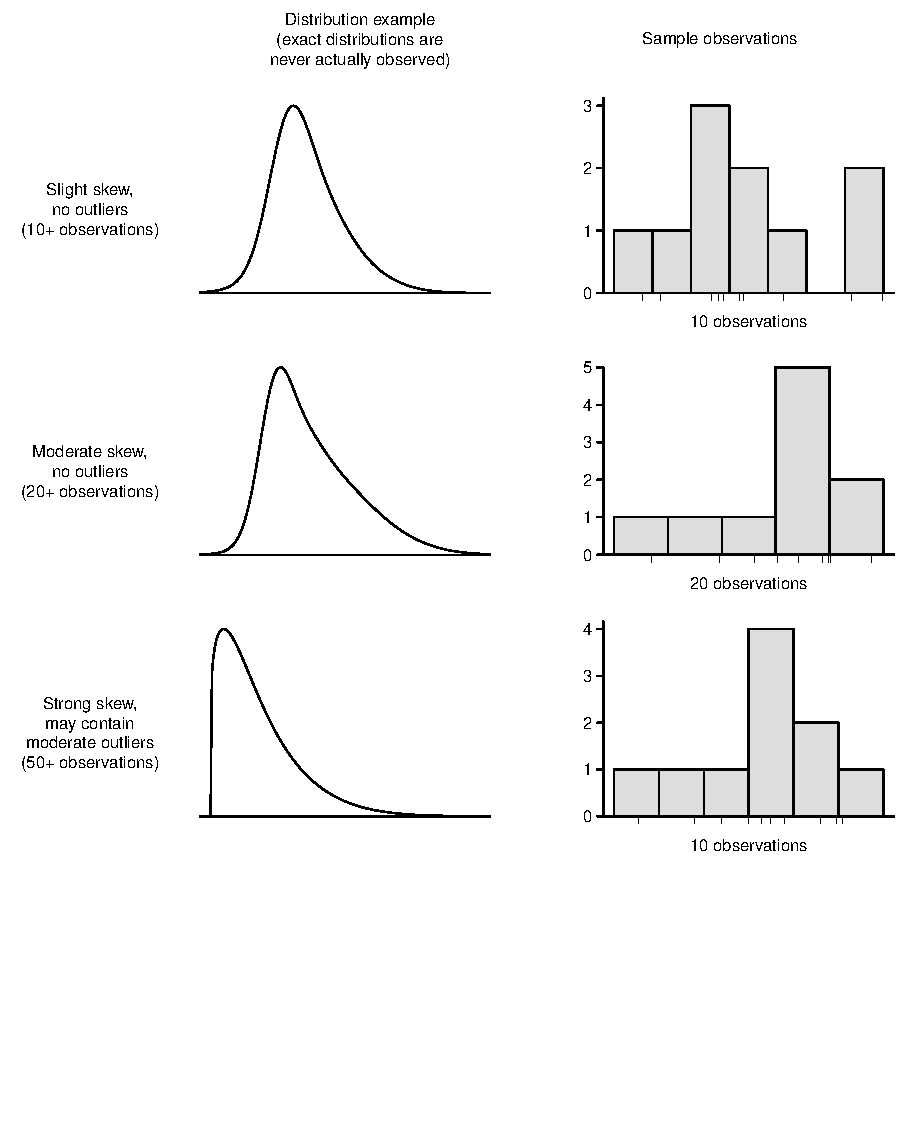
\includegraphics[width=\textwidth]{05/figures/varyingDegreesOfSkew/varyingDegreesOfSkew}
%\caption{12 plots with varying degrees of skewness. Note.}
%\label{varyingDegreesOfSkew}
%\end{figure}
%
%\end{example}

The motivation in Chapter~\ref{foundationsForInference} for requiring a large sample was two-fold. First, a large sample ensures that the sampling distribution of $\bar{x}$ is nearly normal. We will see in Section~\ref{normalityCond} that the new condition introduced above -- that the population data are nearly normal -- resolves this issue. The second motivation for a large sample was that we get a better estimate of the standard error when using a large sample. %, and this topic is discussed in Sections~\ref{introducingTheTDistribution} and~\ref{tDistSolutionToSEProblem}. 
The standard error estimate will not generally be accurate for smaller sample sizes, and this motivates the introduction of the $t$ distribution, which is introduced and applied in Sections~\ref{introducingTheTDistribution}-\ref{oneSampleTTests}.

%. Ultimately, we will use a new distribution called the $t$ distribution in place of the normal distribution. Sections~\ref{oneSampleTConfidenceIntervals} and~\ref{oneSampleTTests} feature how to use the $t$ distribution with confidence intervals and hypothesis testing. %Generally the $t$ distribution is preferred to the normal distribution for any sized sample of numerical data, unless the population standard deviation is known.

%It is useful to revisit our reasons for requiring a large sample for the normal model. We first wanted to ensure the sample mean was nearly normal. Secondly, when the sample size was small, the standard error estimate was not reliable. A sample size of 30 or more helps ensure this error estimate was adequate. We examine these two issues separately, leading us to a new distribution that will be useful for small sample inference about means.

%\subsection{Large sample examples}



\subsection{The normality condition}
\label{normalityCond}

%To apply the inference tools to $\bar{x}$ from a small sample, we require the data come from a nearly normal distribution. Then, w
We use a special case of the Central Limit Theorem to ensure the distribution of the sample means will be nearly normal, regardless of sample size, provided the data come from a nearly normal distribution.

\begin{termBox}{\tBoxTitle{Central Limit Theorem for normal data}
The sampling distribution of the mean is nearly normal when the sample observations are independent and come from a nearly normal distribution. This is true for any sample size.}
\end{termBox}

While this seems like a very helpful special case, there is one small problem. It is inherently difficult to verify normality in small data sets.

\begin{caution}
{Checking the normality condition}
{We should exercise caution when verifying the normality condition for small samples. It is important to not only examine the data but also think about where the data come from. For example, ask: would I expect this distribution to be symmetric, and am I confident that outliers are rare?}
%Always ask: Is it reasonable to assume this type of data are nearly normal?}
\end{caution}

You may relax the normality condition as the sample size goes up. If the sample size is 15 or more, even moderate skew is not a concern. Once the sample size hits about 30 or~40, then we can ignore somewhat strong skew. Cases of very strong skew or the presence of extreme outliers require more careful examination and there are no rules of thumb for a minimum sample size. %In such cases, it is sometimes useful transform the data (see Section~\ref{transformingDataSubsection}).


\subsection{Introducing the $t$ distribution}
\label{introducingTheTDistribution}

We will address the uncertainty of the standard error estimate by using a new distribution: the $t$ distribution. A $t$ distribution, shown as a solid line in Figure~\ref{tDistCompareToNormalDist}, has a bell shape. However, its tails are thicker than the normal model's. 
%This means we would not be as surprised to observe a random variable from the $t$ distribution further from zero than we would from a standard normal model (i.e. $N(0, 1)$).
This means observations are more likely to fall beyond two standard deviations from the mean than under the normal distribution\footnote{The standard deviation of the $t$ distribution is actually a little more than 1. However, it is useful to always think of the $t$ distribution as having a standard deviation of 1 in all of our applications.}.
These extra thick tails are exactly the correction we need to resolve the problem of a poorly estimated standard error.

\begin{figure}
\centering
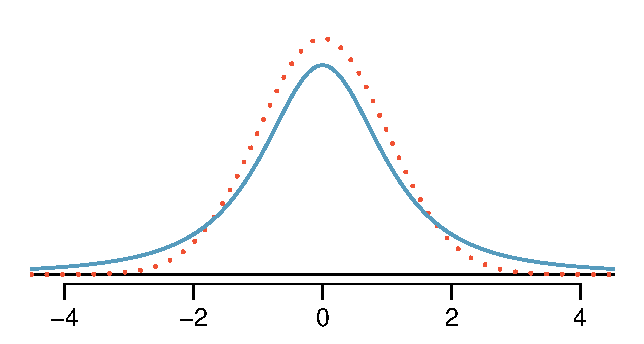
\includegraphics[height=45mm]{06/figures/tDistCompareToNormalDist/tDistCompareToNormalDist}
\caption{Comparison of a $t$ distribution (solid line) and a normal distribution (dotted line).}
\label{tDistCompareToNormalDist}
\end{figure}

%The normal model had two parameters: the mean ($\mu$) and the standard deviation ($\sigma$). 
The $t$ distribution, always centered at zero, has a single parameter: degrees of freedom. The \term{degrees of freedom ($\mathbf{df}$)} describe the exact bell shape of the $t$ distribution. Several $t$ distributions are shown in Figure~\ref{tDistConvergeToNormalDist}. When there are more degrees of freedom, the $t$~distribution looks very much like the standard normal distribution.

\begin{figure}
\centering
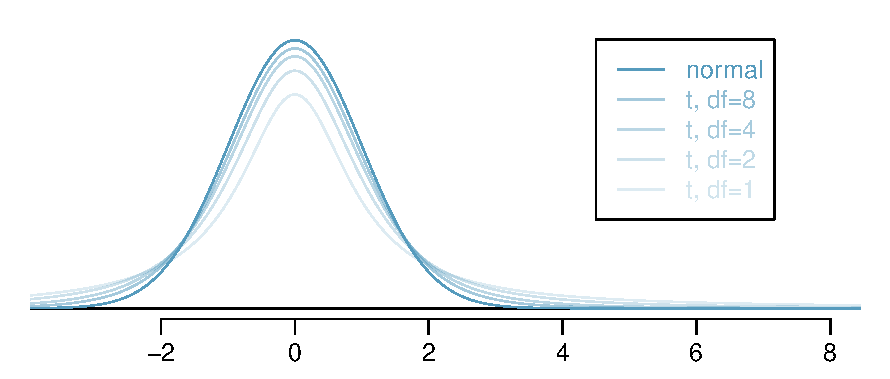
\includegraphics[width=0.7\textwidth]{06/figures/tDistConvergeToNormalDist/tDistConvergeToNormalDist}
\caption{The larger the degrees of freedom, the more closely the $t$ distribution resembles the standard normal model.}\vspace{-2mm}
\label{tDistConvergeToNormalDist}
\end{figure}

\begin{termBox}{\tBoxTitle{Degrees of freedom (df)}
The degrees of freedom describe the shape of the $t$ distribution. The larger the degrees of freedom, the more closely the distribution approximates the normal model.}
\end{termBox}

When the degrees of freedom is about 30 or more, the $t$ distribution is nearly indistinguishable from the normal distribution. In Section~\ref{tDistSolutionToSEProblem}, we relate degrees of freedom to sample size.

We will find it very useful to become familiar with the $t$ distribution, because it plays a very similar role to the normal distribution during inference for small samples of numerical data. %In fact, you should generally favor the use of the $t$ distribution, even when the sample size is 30 or larger.
We use a \term{t table}, partially shown in Table~\ref{tTableSample}, in place of the normal probability table for small sample numerical data. %This table is partially shown in Table~\ref{}. 
A larger table is presented in Appendix~\vref{tDistributionTable}.

\begin{table}[hht]
\centering
\begin{tabular}{r | rrr rr}
one tail & \hspace{1.5mm}  0.100 & \hspace{1.5mm} 0.050 & \hspace{1.5mm} 0.025 & \hspace{1.5mm} 0.010 & \hspace{1.5mm} 0.005  \\
two tails & 0.200 & 0.100 & 0.050 & 0.020 & 0.010 \\
\hline
{$df$} \hfill 1  &  {\normalsize  3.08} & {\normalsize  6.31} & {\normalsize 12.71} & {\normalsize 31.82} & {\normalsize 63.66}  \\ 
2  &  {\normalsize  1.89} & {\normalsize  2.92} & {\normalsize  4.30} & {\normalsize  6.96} & {\normalsize  9.92}  \\ 
3  &  {\normalsize  1.64} & {\normalsize  2.35} & {\normalsize  3.18} & {\normalsize  4.54} & {\normalsize  5.84}  \\ 
$\vdots$ & $\vdots$ &$\vdots$ &$\vdots$ &$\vdots$ & \\
17  &  {\normalsize  1.33} & {\normalsize  1.74} & {\normalsize  2.11} & {\normalsize  2.57} & {\normalsize  2.90}  \\ 
\em\color{tableHLBlue}18  &  \em\color{tableHLBlue}{\normalsize  1.33} & \em\color{tableHLBlue}{\normalsize  1.73} & \em\color{tableHLBlue}{\normalsize  2.10} & \em\color{tableHLBlue}{\normalsize  2.55} & \em\color{tableHLBlue}{\normalsize  2.88}  \\ 
19  &  {\normalsize  1.33} & {\normalsize  1.73} & {\normalsize  2.09} & {\normalsize  2.54} & {\normalsize  2.86}  \\ 
20  &  {\normalsize  1.33} & {\normalsize  1.72} & {\normalsize  2.09} & {\normalsize  2.53} & {\normalsize  2.85}  \\ 
$\vdots$ & $\vdots$ &$\vdots$ &$\vdots$ &$\vdots$ & \\
400  &  {\normalsize  1.28} & {\normalsize  1.65} & {\normalsize  1.97} & {\normalsize  2.34} & {\normalsize  2.59}  \\ 
500  &  {\normalsize  1.28} & {\normalsize  1.65} & {\normalsize  1.96} & {\normalsize  2.33} & {\normalsize  2.59}  \\ 
$\infty$  &  {\normalsize  1.28} & {\normalsize  1.64} & {\normalsize  1.96} & {\normalsize  2.33} & {\normalsize  2.58}  \\ 
\end{tabular}
\caption{An abbreviated look at the $t$ table. Each row represents a different $t$ distribution. The columns describe the tail areas at each standard deviation. The row with $df=18$ has been {\em\color{tableHLBlue}highlighted}.}
\label{tTableSample}
\end{table}

Each row in the $t$ table represents a $t$ distribution with different degrees of freedom. The columns correspond to tail probabilities. For instance, if we know we are working with the $t$ distribution with $df=18$, we can examine row 18, which is highlighted in Table~\ref{tTableSample}. If we want the value in this row that identifies the cutoff for an upper tail of 10\%, we can look in the column where \emph{one tail} is 0.100. This cutoff is 1.33. If we had wanted the cutoff for the lower 10\%, we would use -1.33. Just like the normal distribution, all $t$ distributions are symmetric.

\begin{example}{What proportion of the $t$ distribution with 18 degrees of freedom falls below -2.10?}
Just like a normal probability problem, we first draw the picture in Figure~\ref{tDistDF18LeftTail2Point10} and shade the area below -2.10. To find this area, we identify the appropriate row: $df=18$. Then we identify the column containing the absolute value of -2.10; it is the third column. Because we are looking for just one tail, we examine the top line of the table, which shows that a one tail area for a value in the third row corresponds to 0.025. About 2.5\% of the distribution falls below -2.10. In the next example we encounter a case where the exact $t$ value is not listed in the table.
\end{example}

\begin{figure}
\centering
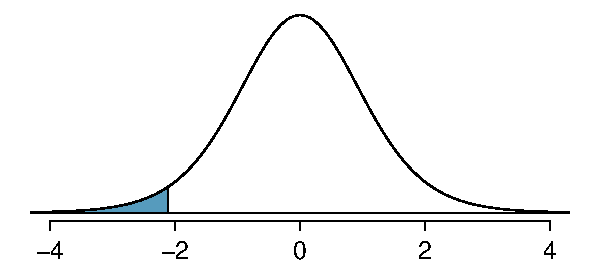
\includegraphics[width=0.51\textwidth]{06/figures/tDistDF18LeftTail2Point10/tDistDF18LeftTail2Point10}
\caption{The $t$ distribution with 18 degrees of freedom. The area below -2.10 has been shaded.}
\label{tDistDF18LeftTail2Point10}
\end{figure}

\begin{example}{A $t$ distribution with 20 degrees of freedom is shown in the left panel of Figure~\ref{tDistDF20RightTail1Point65}. Estimate the proportion of the distribution falling above 1.65.}
We identify the row in the $t$ table using the degrees of freedom: $df=20$. Then we look for 1.65; it is not listed. It falls between the first and second columns. Since these values bound 1.65, their tail areas will bound the tail area corresponding to 1.65. We identify the one tail area of the first and second columns, 0.050 and 0.10, and we conclude that between 5\% and 10\% of the distribution is more than 1.65 standard deviations above the mean. If we like, we can identify the precise area using statistical software: 0.0573.
\end{example}

\begin{figure}
\centering
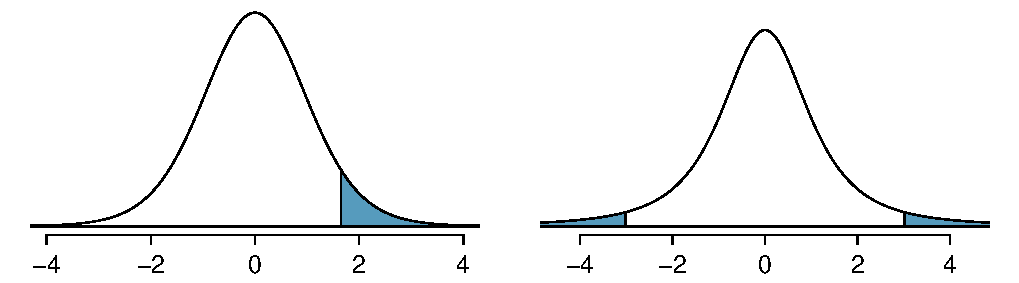
\includegraphics[width=0.85\textwidth]{06/figures/tDistDF20RightTail1Point65/tDistDF20RightTail1Point65}
\caption{Left: The $t$ distribution with 20 degrees of freedom, with the area above 1.65 shaded. Right: The $t$ distribution with 2 degrees of freedom, and the area further than 3 units from 0 has been shaded.}
\label{tDistDF20RightTail1Point65}
\end{figure}

\begin{example}{A $t$ distribution with 2 degrees of freedom is shown in the right panel of Figure~\ref{tDistDF20RightTail1Point65}. Estimate the proportion of the distribution falling more than 3 units from the mean (above or below).}
As before, first identify the appropriate row: $df=2$. Next, find the columns that capture 3; because $2.92 < 3 < 4.30$, we use the second and third columns. Finally, we find bounds for the tail areas by looking at the two tail values: 0.05 and 0.10. We use the two tail values because we are looking for two (symmetric) tails. %\footnote{From a computer: 0.0955.}.
\end{example}

\begin{exercise}
What proportion of the $t$ distribution with 19 degrees of freedom falls above -1.79 units?\footnote{We finding the shaded area \emph{above} -1.79 (we leave the picture to you). The small left tail is between 0.025 and 0.05, so the larger upper region must have an area between 0.95 and 0.975.}
\end{exercise}



\subsection{The $t$ distribution as a solution to the standard error problem}
\label{tDistSolutionToSEProblem}

When estimating the mean and standard error from a small sample, the $t$ distribution is a more accurate tool than the normal model.

\begin{tipBox}{\tipBoxTitle{When to use the $t$ distribution}
When observations are independent and nearly normal, use the $t$ distribution for inference of the sample mean. You may relax the nearly normal condition as the sample size increases. For example, use the $t$ distribution for a sample with size 30 that is strongly skewed.
}
\end{tipBox}

We prefer the $t$ distribution instead of the normal model because we have extra uncertainty in the estimate of the standard error, especially for smaller samples. To proceed with the $t$ distribution for inference about a single mean, we must check two conditions.
\begin{description}
\item[Independence of observations.] We verify this condition just as we did before. We collect a simple random sample from less than 10\% of the population, or if it was an experiment or random process, carefully ensure to the best of our abilities that the observations were independent.
\item[Observations come from a nearly normal distribution.] This second condition is difficult to verify with small data sets. We often (i) take a look at a plot of the data for obvious departures from the normal model and (ii) consider whether any previous experiences alert us that the data may not be nearly normal.
\end{description}
%As the sample size becomes larger, we may relax the normality condition. For instance, if the sample size is 30 or more, we can use the $t$ distribution with data so long as it is not extremely skewed. This actually replaces 
When examining a sample mean and estimated standard error from a sample of $n$ independent and nearly normal observations, we will use a $t$ distribution with $n-1$ degrees of freedom ($df$). For example, if the sample size was 19, then we would use the $t$ distribution with $df=19-1=18$ degrees of freedom and proceed exactly as we did in Chapter~\ref{foundationsForInference}, except that \emph{now we use the $t$ table}.

We can relax the normality condition for the observations when the sample size becomes large. For instance, a slightly skewed data set might be acceptable if there were at least 15 observations. A strongly skewed data set would require about 30 observations. For an extremely skewed data set, perhaps 100 or more. When very extreme outliers are present, proceed with extra caution.


\subsection{One sample $t$ confidence intervals}
\label{oneSampleTConfidenceIntervals}

Dolphins are at the top of the oceanic food chain, which causes dangerous substances such as mercury to concentrate in their organs and muscles. This is an important problem for both dolphins and other animals, like humans, who occasionally eat them. For instance, this is particularly relevant in Japan where school meals have included dolphin at times.
\setlength{\captionwidth}{71.5mm}

\begin{figure}[h]
\centering
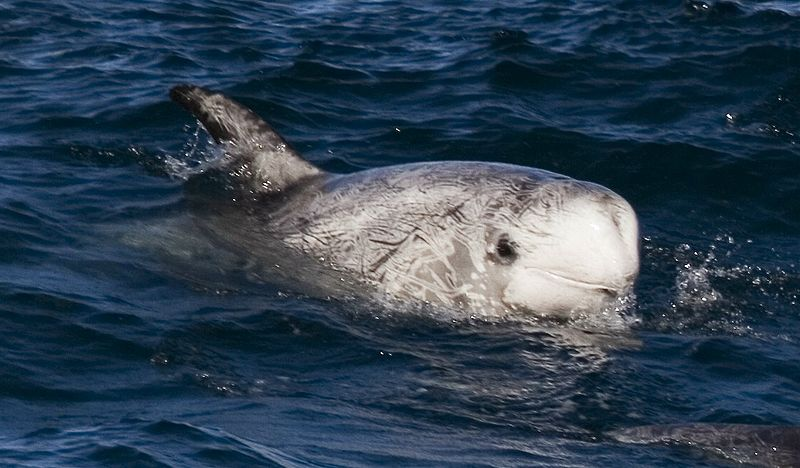
\includegraphics[width=71.5mm]{06/figures/rissosDolphin.jpg}  \\
\addvspace{2mm}
\begin{minipage}{\textwidth}
   \caption[rissosDolphinPic]{A Risso's dolphin.\vspace{-1mm} \\
   -----------------------------\vspace{-2mm}\\
   {\footnotesize Photo by Mike Baird (\urlwofont{http://www.bairdphotos.com/}).%Image is under Creative Commons Attribution 2.0 Generic.
}\vspace{-8mm}}
   \label{rissosDolphin}
\end{minipage}
\vspace{3mm}
%\begin{minipage}{\textwidth}
%\caption[rissosDolphinPic]{A Risso's dolphin\vspace{-3mm}\footnote{Photo by Mike Baird. Image is under Creative Commons Attribution 2.0 Generic.\vspace{2mm}}.}
%\end{minipage}
\end{figure}
\setlength{\captionwidth}{\mycaptionwidth}

Here we identify a confidence interval for the average mercury content in dolphin muscle using a sample of 19 Risso's dolphins from the Taiji area in Japan\footnote{Taiji was featured in the movie \emph{The Cove}, and it is a significant source of dolphin and whale meat in Japan. Thousands of dolphins pass through the Taiji area annually, and we will assume these 19 dolphins represent a simple random sample from those dolphins. Data reference: Endo T and Haraguchi K. 2009. High mercury levels in hair samples from residents of Taiji, a Japanese whaling town. Marine Pollution Bulletin 60(5):743-747.}. The data are summarized in Table~\ref{summaryStatsOfHgInMuscleOfRissosDolphins}. The minimum and maximum observed values can be used to evaluate whether or not there are any extreme outliers or obvious skew.

\begin{table}[h]
\centering
\begin{tabular}{ccc cc}
\hline
$n$ & $\bar{x}$ & $s$ & minimum & maximum \\
19   & 4.4	  & 2.3  & 1.7	       & 9.2 \\
\hline
\end{tabular}
\caption{Summary of mercury content in the muscle of 19 Risso's dolphins from the Taiji area. Measurements are in $\mu$g/wet g (micrograms of mercury per wet gram of muscle).}
\label{summaryStatsOfHgInMuscleOfRissosDolphins}
\end{table}

\begin{example}{
%Evaluate the independence and normality conditions for applying the $t$ distribution to the sample mean and estimated standard error.
Are the independence and normality conditions satisfied for this data~set?}
The observations are a simple random sample and consist of less than 10\% of the population, therefore independence is reasonable. The summary statistics in Table~\ref{summaryStatsOfHgInMuscleOfRissosDolphins} do not suggest any strong skew or outliers; all observations are within 2.5 standard deviations of the mean. Based on this evidence, the normality assumption seems reasonable.
\end{example}

In the normal model, we used $z^{\star}$ and the standard error to determine the width of a confidence interval. We revise the confidence interval formula slightly when using the $t$ distribution:
\begin{eqnarray*}
\bar{x} \ \pm\  t^{\star}_{df}SE
\end{eqnarray*}
\marginpar[\raggedright\vspace{-9mm}

$t^{\star}_{df}$\vspace{1mm}\\\footnotesize Multiplication\\factor for\\$t$ conf. interval]{\raggedright\vspace{-9mm}

$t^{\star}_{df}$\vspace{1mm}\\\footnotesize Multiplication\\factor for\\$t$ conf. interval}The sample mean and estimated standard error are computed just as before ($\bar{x} = 4.4$ and $SE = s/\sqrt{n} = 0.528$). The value $t^{\star}_{df}$ is a cutoff we obtain based on the confidence level and the $t$ distribution with $df$ degrees of freedom. Before determining this cutoff, we will first need the degrees of freedom.
%However, we must now identify $t^{\star}_{df}$ instead of $z^{\star}$ for the confidence interval.
%We first identify the degrees of freedom associated with the appropriate $t$ distribution (row $df=18$ in the $t$ table). Then determine the column corresponding to 95\% confidence (two tails: 0.05 for 95\% confidence). Then $t^{\star}_{df}$ is the intersection of this row and column in the $t$ table. 

\begin{termBox}{\tBoxTitle{Degrees of freedom for a single sample}
If the sample has $n$ observations and we are examining a single mean, then we use the $t$ distribution with $df=n-1$ degrees of freedom.}
\end{termBox}

In our current example, we should use the $t$ distribution with $df=19-1=18$ degrees of freedom. Then identifying $t_{18}^{\star}$ is similar to how we found $z^{\star}$. 
\begin{itemize}
\setlength{\itemsep}{0mm}
\item For a 95\% confidence interval, we want to find the cutoff $t^{\star}_{18}$ such that 95\% of the $t$ distribution %($df = 18$)
is between -$t^{\star}_{18}$ and $t^{\star}_{18}$.
\item We look in the $t$ table on page~\pageref{tTableSample}, find the column with area totaling 0.05 in the two tails (third column), and then the row with 18 degrees of freedom: $t^{\star}_{18} = 2.10$.
\end{itemize}
Generally the value of $t^{\star}_{df}$ is slightly larger than what we would expect under the normal model with~$z^{\star}$.



Finally, we can substitute all our values into the confidence interval equation to create the 95\% confidence interval for the average mercury content in muscles from Risso's dolphins that pass through the Taiji area:
\begin{eqnarray*}
\bar{x} \ \pm\  t^{\star}_{18}SE
	\quad \to \quad
4.4 \ \pm\  2.10 \times 0.528
	\quad \to \quad
(3.87, 4.93)
\end{eqnarray*}
We are 95\% confident the average mercury content of muscles in Risso's dolphins is between 3.87 and 4.93 $\mu$g/wet gram. This falls above the US safety limit, which is 0.5 $\mu$g per wet gram\footnote{\href{http://www.ban.org/ban-hg-wg/Mercury.ToxicTimeBomb.Final.PDF}{www.ban.org/ban-hg-wg/Mercury.ToxicTimeBomb.Final.PDF}}.

\begin{termBox}{\tBoxTitle{Finding a $t$ confidence interval for the mean}
Based on a sample of $n$ independent and nearly normal observations, a confidence interval for the population mean is
\begin{eqnarray*}
\bar{x} \ \pm\  t^{\star}_{df}SE
\end{eqnarray*}
where $\bar{x}$ is the sample mean, $t^{\star}_{df}$ corresponds to the confidence level and degrees of freedom, and $SE$ is the standard error as estimated by the sample.}
\end{termBox}

\begin{exercise} \label{croakerWhiteFishPacificExerConditions}
The FDA's webpage provides some data on mercury content of fish\footnote{http://www.fda.gov/Food/FoodSafety/Product-SpecificInformation/Seafood/\\ FoodbornePathogensContaminants/Methylmercury/ucm115644.htm}. Based on a sample of 15 croaker white fish (Pacific), a sample mean and standard deviation were computed as 0.287 and 0.069 ppm (parts per million), respectively. The 15 observations ranged from 0.18 to 0.41 ppm. We will assume these observations are independent. Based on the summary statistics of the data, do you have any objections to the normality condition of the individual observations?\footnote{There are no extreme outliers; all observations are within 2 standard deviations of the mean. If there is skew, it is not evident. There are no red flags for the normal model based on this (limited) information, and we do not have reason to believe the mercury content is not nearly normal in this type of fish.}
\end{exercise}

\begin{example}{Estimate the standard error of $\bar{x}=0.287$ ppm from the statistics in Exercise~\exer{croakerWhiteFishPacificExerConditions}. If we are to use the $t$ distribution to create a 90\% confidence interval for the actual mean of the mercury content, identify the degrees of freedom we should use and also find $t^{\star}_{df}$.}
\label{croakerWhiteFishPacificExerSEDFTStar}
The standard error: $SE = \frac{0.069}{\sqrt{15}} = 0.0178$. Degrees of freedom: $df = n - 1 = 14$.

Looking in the column where two tails is 0.100 (since we want a 90\% confidence interval) and row $df=14$, we identify $t^{\star}_{14} = 1.76$.
\end{example}

\begin{exercise}
Based on the results of Exercise~\exer{croakerWhiteFishPacificExerConditions} and Example~\exam{croakerWhiteFishPacificExerSEDFTStar}, compute a 90\% confidence interval for the average mercury content of croaker white fish (Pacific).\footnote{Use $\bar{x} \pm t^{\star}_{14} SE$: $0.287 \pm 1.76\times 0.0178$. This corresponds to $(0.256, 0.318)$. We are 90\% confident that the average mercury content of croaker white fish (Pacific) is between 0.256 and 0.318 ppm.}
\end{exercise}



\subsection{One sample $t$ tests}
\label{oneSampleTTests}

An SAT preparation company claims that its students' scores improve by over 100 points on average after their course. A consumer group would like to evaluate this claim, and they collect data on a random sample of 30 students who took the class. Each of these students took the SAT before and after taking the company's course, and so we have a difference in scores for each student. We will examine these differences $x_1=57$, $x_2=133$, ..., $x_{30}=140$ as a sample to evaluate the company's claim. 
(These are called \emph{paired data}, which is a topic we will discuss further in Section~\ref{pairedData}.) 
The distribution of the difference in scores, shown in Figure~\ref{satImprovementHTDataHistogram}, has mean 135.9 and standard deviation 82.2. Do these data provide convincing evidence to back up the company's claim? 

\begin{figure}
\centering
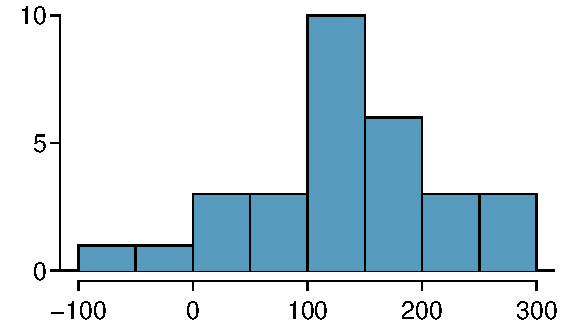
\includegraphics[width=0.54\textwidth]{06/figures/satImprovementHTDataHistogram/satImprovementHTDataHistogram}
\caption{Sample distribution of improvements in SAT scores after taking the SAT course.}
\label{satImprovementHTDataHistogram}
\end{figure}

\begin{exercise}
Set up hypotheses to evaluate the company's claim. Use $\mu$ to represent the true average difference in student scores.\footnote{This is a one-sided test. $H_0$: student scores do not improve by more than 100 after taking the company's course. $\mu \leq 100$ (or simply $\mu = 100$). $H_A$: students scores improve by more than 100 points on average after taking the company's course. $\mu > 100$.}
\end{exercise}

\begin{exercise}
Are the conditions to use the $t$ distribution method satisfied?\footnote{This is a random sample from less than 10\% of the company's students (assuming they have more than 300 former students), so the independence condition is reasonable. The normality condition also seems reasonable based on Figure~\ref{satImprovementHTDataHistogram}. We can use the $t$ distribution method.}
\end{exercise}

Just as we did for the normal case, we standardize the sample mean using the Z score to identify the test statistic. However, we will write $T$\marginpar[\raggedright$T$\vspace{0.5mm}\\\footnotesize T score\\(like Z score)]{\raggedright$T$\vspace{0.5mm}\\\footnotesize T score\\(like Z score)} instead of $Z$, because we have a small sample and are basing our inference on the $t$ distribution:
\begin{eqnarray*}
T = \frac{\bar{x} - \text{null value}}{SE} = \frac{135.9 - 100}{82.2/\sqrt{30}} = 2.39
\end{eqnarray*}
If the null hypothesis was true, the test statistic $T$ would follow a $t$ distribution with $df = n-1 = 29$ degrees of freedom. We can draw a picture of this distribution and mark the observed $T$, as in Figure~\ref{pValueShownForSATHTOfOver100PtGain}. The shaded right tail represents the p-value: the probability of observing such strong evidence in favor of the SAT company's claim, if the average student improvement is really only 100.

\begin{figure}
\centering
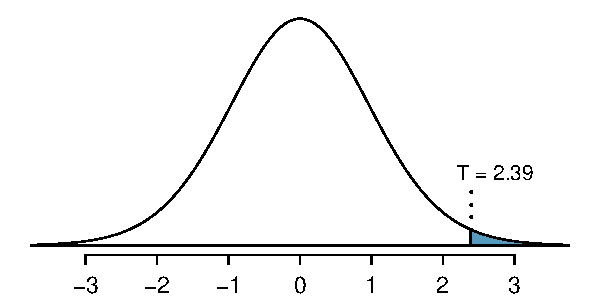
\includegraphics[width=0.65\textwidth]{06/figures/pValueShownForSATHTOfOver100PtGain/pValueShownForSATHTOfOver100PtGain}
\caption{The $t$ distribution with 29 degrees of freedom.}
\label{pValueShownForSATHTOfOver100PtGain}
\end{figure}

\begin{exercise}
Use the $t$ table in Appendix~\vref{tDistributionTable} to identify the p-value. What do you conclude?\footnote{We use the row with 29 degrees of freedom. The value $T=2.39$ falls between the third and fourth columns. Because we are looking for a single tail, this corresponds to a p-value between 0.01 and 0.025. The p-value is guaranteed to be less than 0.05 (the default significance level), so we reject the null hypothesis. The data provide convincing evidence to support the company's claim that student scores improve by more than 100 points following the class.}
\end{exercise}

\begin{exercise}
Because we rejected the null hypothesis, does this mean that taking the company's class improves student scores by more than 100 points on average?\footnote{This is an observational study, so we cannot make this causal conclusion. For instance, maybe SAT test takers tend to improve their score over time even if they don't take a special SAT class, or perhaps only the most motivated students take such SAT courses.}
\end{exercise}



%==========
\section{Paired data}
\label{pairedData}

Are textbooks actually cheaper online? Here we compare the price of textbooks at UCLA's bookstore and prices at Amazon.com. Seventy-three UCLA courses were randomly sampled in Spring 2010, representing less than 10\% of all UCLA courses\footnote{When a class had multiple books, only the most expensive text was considered.}. A portion of this \data{textbooks} data set is shown in Table~\ref{textbooksDF}. \vspace{2.5mm}

\begin{table}[h]
\centering
\begin{tabular}{rllrrr}
  \hline
 & deptAbbr & course & uclaNew & amazNew & diff \\ 
  \hline
1 & Am Ind &  C170 & 27.67 & 27.95 & -0.28 \\ 
  2 & Anthro & 9 & 40.59 & 31.14 & 9.45 \\ 
$\vdots$ & $\vdots$ & $\vdots$ & $\vdots$ & $\vdots$ & $\vdots$ \\
%  72 & Wom Std & M144 & 23.76 & 18.72 & 5.04 \\ 
  73 & Wom Std & 285 & 27.70 & 18.22 & 9.48 \\ 
   \hline
\end{tabular}
\caption{Three cases of the \data{textbooks} data set.}
\label{textbooksDF}
\end{table}\vspace{-2.5mm}


\subsection{Paired observations and samples}

Each textbook has two corresponding prices in the data set: one for the UCLA bookstore and one for Amazon. Therefore, each textbook price from the UCLA bookstore has a natural correspondence with a textbook price from Amazon. When two sets of observations have this special correspondence, they are said to be \term{paired}.

\begin{termBox}{\tBoxTitle{Paired data}
Two sets of observations are \emph{paired} if each observation in one set has a special correspondence or connection with exactly one observation in the other data set.}
\end{termBox}

To analyze paired data, it is often useful to look at the difference in outcomes of each pair of observations. In the \data{textbook} data set, we look at the difference in prices, which is represented as the \var{diff} variable in the \data{textbooks} data. Here the differences are taken as
\begin{eqnarray*}
\text{UCLA price} - \text{Amazon price}
\end{eqnarray*}
for each book. It is important that we always subtract using a consistent order; here Amazon prices are always subtracted from UCLA prices. A histogram of these differences is shown in Figure~\ref{diffInTextbookPricesS10}, which exhibits moderate skew. Using differences between paired observations is a common and useful way to analyze paired data. %, and something we first saw in Section~\ref{oneSampleTTests}.

\begin{figure}
\centering
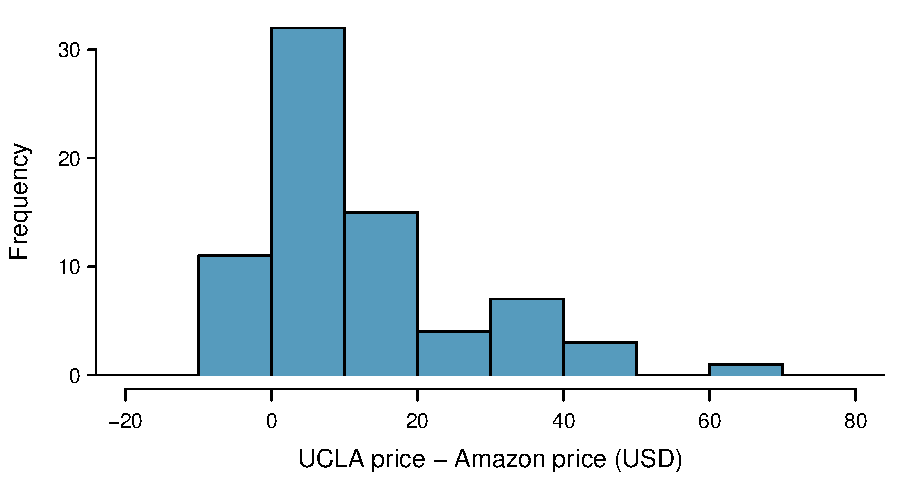
\includegraphics[width=0.8\textwidth]{05/figures/textbooksS10/diffInTextbookPricesS10}
\caption{Histogram of the difference in price for each book sampled.}
\label{diffInTextbookPricesS10}
\end{figure}

\begin{exercise}
The first difference shown in Table~\ref{textbooksDF} is computed as $27.67-27.95=-0.28$. Verify the other two differences in the table are computed correctly.
\end{exercise}


\subsection{Inference for paired data}

To analyze a paired data set, we use our inference framework and we simply apply them to the differences in the paired observations. %We will apply the $t$ distribution for $\bar{x}_{diff}$, but it would be okay to use the normal model for such a large sample.

\begin{table}[hh]
\centering
\begin{tabular}{ccccc}
\hline
$n_{_{diff}}$	&\hspace{3mm}& $\bar{x}_{_{diff}}$	&\hspace{3mm}& $s_{_{diff}}$ \vspace{1mm}\\
73			&& 12.76				&& 14.26 \\
\hline
\end{tabular}
\caption{Summary statistics for the \var{diff} variable. There were 73 books, so there are 73 differences.}
\label{textbooksSummaryStats}
\end{table}

\begin{example}{Set up and implement a hypothesis test to determine whether, on average, there is a difference between Amazon's price for a book and the UCLA bookstore's price.}
\label{htForDiffInUCLAAndAmazonTextbookPrices}
There are two scenarios: there is no difference or there is a difference in average prices. The \emph{no difference} scenario is always the null hypothesis:
\begin{itemize}
\item[$H_0$:] $\mu_{diff}=0$. There is no difference in the average textbook price. The notation $\mu_{diff}$ is used as a notational reminder that we should only work with the difference in prices.
\item[$H_A$:] $\mu_{diff} \neq 0$. There is a difference in average prices.
\end{itemize}
Can the $t$ distribution be used to describe the sampling distribution of $\bar{x}_{diff}$? We must check that the differences meet the conditions. The observations are based on a simple random sample from less than 10\% of all books sold at the bookstore, so independence is reasonable. Additionally, the skew is only moderate, which is okay for such a large sample ($n=73$). Thus, we can use the $t$ distribution to model the sampling distribution of $\bar{x}_{diff}$.

We compute the standard error associated with $\bar{x}_{diff}$ using the standard deviation of the differences and the number of differences:
$$SE_{\bar{x}_{diff}} = \frac{s_{diff}}{\sqrt{n_{diff}}} = \frac{14.26}{\sqrt{73}} = 1.67$$
To visualize the p-value, the sampling distribution of $\bar{x}_{diff}$ is drawn under the condition as though $H_0$ was true, which is shown in Figure~\ref{textbooksS10HTTails}. The p-value is represented by the two (very) small tails.

\begin{figure}
\centering
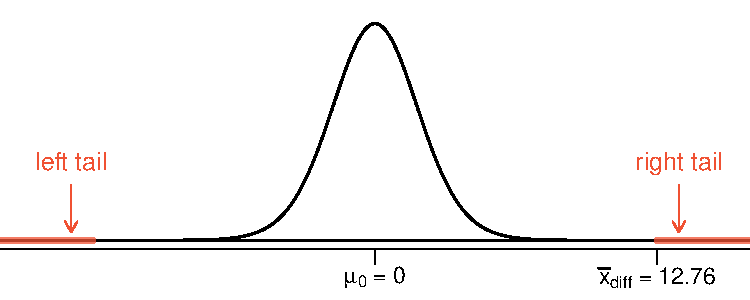
\includegraphics[width=0.65\textwidth]{05/figures/textbooksS10/textbooksS10HTTails}
\caption{Sampling distribution for the mean difference in book prices, if the true average difference is zero.}
\label{textbooksS10HTTails}
\end{figure}

To find the tail areas, we compute the test statistic, which is the T score of $\bar{x}_{diff}$ under the condition $\mu_{diff} = 0$:
$$T = \frac{\bar{x}_{diff} - 0}{SE_{x_{diff}}} = \frac{12.76 - 0}{1.67} = 7.59$$
We can look for $T=7.59$ in row $df=73-1=72$ in the $t$ table in Appendix~\vref{tDistributionTable}; since this row isn't available, we can examine the next smaller degree of freedom row: $df=70$. $T=7.59$ is larger than the last column in this row, indicating the p-value is smaller than 0.01 (two tails!).
%This T score is so large it isn't even in the table, which ensures the single tail area will be 0.0002 or smaller. Since the p-value is both tails and the normal distribution is symmetric, the p-value can be estimated as twice the one-tail area:
%$$\text{p-value} = 2\times (\text{one tail area}) \approx 2\times 0.0002 = 0.0004$$
Because the p-value is less than 0.05, we reject the null hypothesis. We have found convincing evidence that Amazon is, on average, cheaper than the UCLA bookstore for UCLA course textbooks.
\end{example}

The sample size for the paired data was quite large: $n = 73 \geq 30$. For this reason, we could have used the normal model if we prefered, and the results and conclusion would be nearly identical.

\begin{exercise}
Create a 95\% confidence interval for the average price difference between books at the UCLA bookstore and books on Amazon.\footnote{Conditions have already verified and the standard error computed in Example~\exam{htForDiffInUCLAAndAmazonTextbookPrices}. To find the interval, identify $t^{\star}_{70}$ (1.99 for 95\% confidence, i.e. 0.05 in two tails) and plug it, the point estimate, and the standard error into the confidence interval formula:
$$\text{point estimate} \pm t_{70}^{\star}SE \quad\to\quad 12.76 \pm (1.99)(1.67) \quad\to\quad (9.44, 16.08)$$
We are 95\% confident that Amazon is, on average, between \$9.44 and \$16.08 cheaper than the UCLA bookstore for UCLA course books. Had we used the normal model instead, we would have obtained an interval $(9.49, 16.03)$.}
\end{exercise}

\section{Difference of two means}
\label{differenceOfTwoMeans}

In this section we consider a difference in two population means, $\mu_1 - \mu_2$, under the condition that the data are not paired. The methods are similar in theory but different in the details. Just as with a single sample, we identify conditions to ensure a point estimate of the difference, $\bar{x}_1 - \bar{x}_2$, is nearly normal. Next we introduce a formula for the standard error. With these two pieces of information, we will be able to apply the $t$ distribution for calculating confidence intervals and performing hypothesis tests.

We apply these methods to two examples: participants in the 2009 Cherry Blossom Run and newborn infants. This section is motivated by questions like ``Is there convincing evidence that newborns from mothers who smoke have a different average birth weight than newborns from mothers who don't smoke?''

\subsection{Point estimates and standard errors for difference of means}

We would like to estimate the average difference in run times for men and women using a random sample of 45 men and 55 women from the \data{run10} population. Table~\ref{cherryBlossomRun2009SampleOf180SummaryStats} presents relevant summary statistics, and box plots of each sample are shown in Figure~\ref{cbrRunTimesMenWomen}.

\begin{table}[h]
\centering
\begin{tabular}{l rr}
\hline
	&	men	&	women \\
\hline
$\bar{x}$	& 87.56	& 102.04 \\
$s$	&	15.53	& 15.24 \\
$n$	&	45		& 55    \\
\hline
\end{tabular}
\caption{Summary statistics for the run time of 180 participants in the 2009 Cherry Blossom Run.}
\label{cherryBlossomRun2009SampleOf180SummaryStats}
\end{table}
%library(openintro); data(run10Samp); d <- run10Samp; by(d$time, d$gender, mean); by(d$time, d$gender, sd); by(d$time, d$gender, length)

\begin{figure}
\centering
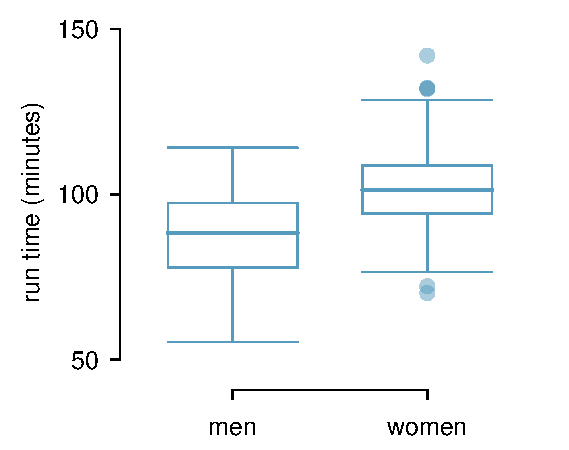
\includegraphics[width=0.5\textwidth]{05/figures/cbrRunTimesMenWomen/cbrRunTimesMenWomen}
\caption{Side-by-side box plots for the sample of 2009 Cherry Blossom Run participants.}
\label{cbrRunTimesMenWomen}
\end{figure}

The two samples are independent of one-another, so the data are not paired. Instead a point estimate of the difference in average 10 mile times for men and women, $\mu_w - \mu_m$, can be found using the two sample means:
\begin{eqnarray*}
\bar{x}_{w} - \bar{x}_{m}\ =\ 102.04 - 87.56\ =\ 14.48
\end{eqnarray*}
Each sample separately satisfies the conditions for using the $t$ distribution: each is a simple random sample from less than 10\% of the population, and each distribution is approximately symmetric. Thus, each sample mean should be nearly normal. Finally, because each sample is independent of the other (e.g. the data are not paired), the difference in sample means can be modeled using a $t$ distribution\footnote{This is a result of probability theory. Because each sample mean is nearly normal and observations in the samples are independent, we are assured the difference is also nearly normal.}.

\begin{termBox}{\tBoxTitle{Conditions for normality of $\bar{x}_1 - \bar{x}_2$}
If the sample means, $\bar{x}_1$ and $\bar{x}_2$, each meet the criteria for having nearly normal sampling distributions and the observations in the two samples are independent, then the difference in sample means, $\bar{x}_1 - \bar{x}_2$, will have a sampling distribution that is nearly normal.}
\end{termBox}

We can quantify the variability in the point estimate, $\bar{x}_{w} - \bar{x}_{m}$, using the following formula for its standard error:
\begin{eqnarray*}
SE_{\bar{x}_{w} - \bar{x}_{m}} = \sqrt{\frac{\sigma_{w}^2}{n_{w}} + \frac{\sigma_{m}^2}{n_{m}}}
\end{eqnarray*}
We usually estimate this standard error using standard deviation estimates  based on the samples:
\begin{align*}
SE_{\bar{x}_{w} - \bar{x}_{m}}
	&= \sqrt{\frac{\sigma_{w}^2}{n_{w}} + \frac{\sigma_{m}^2}{n_{m}}} \\
	&\approx \sqrt{\frac{s_{w}^2}{n_{w}} + \frac{s_{m}^2}{n_{m}}}
	= \sqrt{\frac{13.7^2}{80} + \frac{15.7^2}{100}} = 2.19
\end{align*}
Because each sample has at least 30 observations ($n_{w} = 80$ and $n_{m} = 100$), this substitution using the sample standard deviation tends to be very good.

\begin{termBox}{\tBoxTitle{Distribution of a difference of sample means}
The sample difference of two means, $\bar{x}_1 - \bar{x}_2$, is nearly normal with mean $\mu_{1}-\mu_{2}$ and estimated standard error
\begin{eqnarray}
\textstyle
SE_{\bar{x}_{1} - \bar{x}_{2}} = \sqrt{\frac{s_1^2}{n_1} + \frac{s_2^2}{n_2}}
\label{seOfDifferenceInMeans}
\end{eqnarray}
when each sample mean is nearly normal and all observations are independent.}
\end{termBox}

\subsection{Confidence interval for the difference}

When the conditions are met for the sampling distribution of $\bar{x}_{1} - \bar{x}_{2}$ to be nearly normal, we can construct a 95\% confidence interval for the difference in two means from the framework built in Chapter~\ref{foundationsForInference}. Here a point estimate, $\bar{x}_{w} - \bar{x}_{m} = 8.20$, is associated with a normal model with standard error $SE=2.19$. Using this information, the general confidence interval formula may be applied in an attempt to capture the true difference in means:
\begin{eqnarray*}
\text{point estimate} \pm z^{\star}SE \quad\to\quad 8.20 \pm 1.96\times 2.19 \quad\to\quad (3.91, 12.49)
\end{eqnarray*}
Based on the samples, we are 95\% confident that men ran, on average, between 3.91 and 12.49 minutes faster than women in the 2009 Cherry Blossom Run.

\begin{exercise}
What does 95\% confidence mean? Answer in the footnote\footnote{If we were to collected many such samples and create 95\% confidence intervals for each, then about 95\% of these intervals would contain the population difference, $\mu_w - \mu_m$.}.
\end{exercise}

\begin{exercise}
We may be interested in a different confidence level. Construct the 99\% confidence interval for the population difference in average run times based on the sample data. Hint in the footnote\footnote{The only thing that changes is $z^{\star}$: we use $z^{\star}=2.58$ for a 99\% confidence level. If the selection of $z^{\star}$ is confusing, see Section~4.2.4 for an explanation.}.
\end{exercise}

\subsection{Hypothesis tests based on a difference in means}

A data set called \data{babySmoke} represents a random sample of 150 cases of mothers and their newborns in North Carolina over a year. Four cases from this data set are represented in Table~\ref{babySmokeDF}. We are particularly interested in two variables: \var{weight} and \var{smoke}. The \var{weight} variable represents the weights of the newborns and the \var{smoke} variable describes which mothers smoked during pregnancy. We would like to know if there is convincing evidence that newborns from mothers who smoke have a different average birth weight than newborns from mothers who don't smoke? We will answer this question using a hypothesis test. The smoking group includes 50 cases and the nonsmoking group contains 100 cases, represented in Figure~\ref{babySmokePlotOfTwoGroupsToExamineSkew}.

\begin{table}[h]
\centering
\begin{tabular}{rrrrrll}
  \hline
 & fAge & mAge & weeks & weight & sexBaby & smoke \\ 
  \hline
1 & NA & 13 &  37 & 5.00 & female & nonsmoker \\ 
  2 & NA & 14 &  36 & 5.88 & female & nonsmoker \\ 
  3 & 19 & 15 &  41 & 8.13 & male & smoker \\ 
  $\vdots$ &   $\vdots$ &   $\vdots$ &   $\vdots$ &   $\vdots$ &   $\vdots$ \\
  150 & 45 & 50 &  36 & 9.25 & female & nonsmoker \\ 
   \hline
\end{tabular}
\caption{Four cases from the \data{babySmoke} data set. An observation listed as ``NA'' means that particular piece of data is missing.}
\label{babySmokeDF}
\end{table}

\begin{figure}[h]
\centering
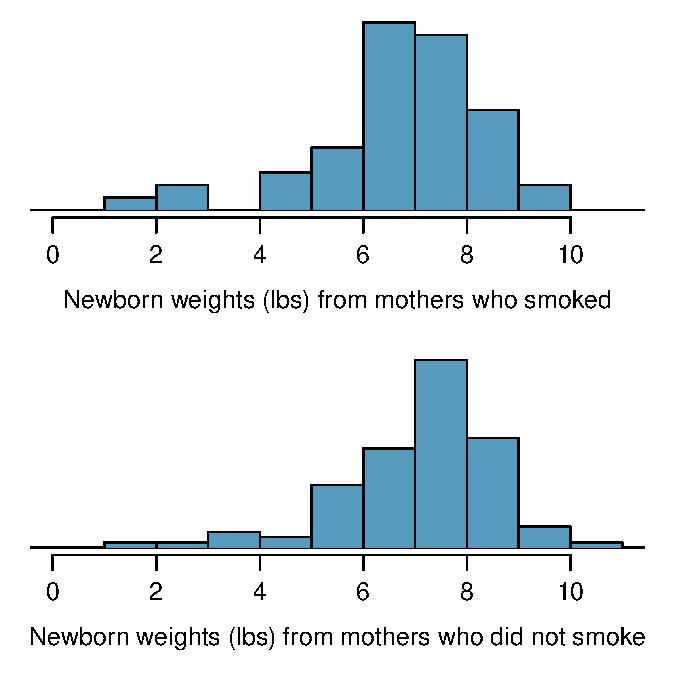
\includegraphics[width=0.6\textwidth]{05/figures/babySmokePlotOfTwoGroupsToExamineSkew/babySmokePlotOfTwoGroupsToExamineSkew}
\caption{The top panel represents birth weights for infants whose mothers smoked. The bottom panel represents the birth weights for infants whose mothers who did not smoke.}
\label{babySmokePlotOfTwoGroupsToExamineSkew}
\end{figure}

\begin{example}{Set up appropriate hypotheses to evaluate whether there is a relationship between a mother smoking and average birth weight.}\label{babySmokeHTForWeight}
The null hypothesis represents the case of no difference between the groups.
\begin{itemize}
\setlength{\itemsep}{0mm}
\item[$H_0$:] There is no difference in average birth weight for newborns from mothers who did and did not smoke. In statistical notation: $\mu_{n} - \mu_{s} = 0$, where $\mu_{n}$ represents non-smoking mothers and $\mu_s$ represents mothers who smoked.
\item[$H_A$:] there is some difference in average newborn weights from mothers who did and did not smoke ($\mu_{n} - \mu_{s} \neq 0$).
\end{itemize}
\end{example}

Summary statistics are shown for each sample in Table~\ref{summaryStatsOfBirthWeightForNewbornsFromSmokingAndNonsmokingMothers}. Because each sample is simple random and consists of less than 10\% of all such cases, the observations are independent. Additionally, each sample size is at least 30 and neither sample distribution is strongly skewed (see Figure~\ref{babySmokePlotOfTwoGroupsToExamineSkew}), so both sample means are associated with a nearly normal distribution.

\begin{table}[h]
\centering
\begin{tabular}{lrr}
	& \resp{smoker} & \resp{nonsmoker} \\
\hline
mean & 6.78 & 7.18 \\
st. dev. & 1.43 & 1.60 \\
samp. size & 50 & 100 \\
\hline
\end{tabular}
\caption{Summary statistics for the \data{babySmoke} data set.}
\label{summaryStatsOfBirthWeightForNewbornsFromSmokingAndNonsmokingMothers}
\end{table}

\begin{exercise} \label{pointEstimateDistributionAndSEForBabySmokeData}
(a)~What is the point estimate of the population difference, $\mu_{n} - \mu_{s}$? (b)~Can we use a normal distribution to model this difference? (c)~Compute the standard error of the point estimate from part (a). Answers in the footnote\footnote{(a)~The difference in sample means is an appropriate point estimate: $\bar{x}_{n} - \bar{x}_{s} = 0.40$. (b)~Because the samples are independent and each sample mean is nearly normal, their difference is also nearly normal. (c)~The standard error of the estimate can be estimated using Equation~(\ref{seOfDifferenceInMeans}):
\begin{eqnarray*}
SE = \sqrt{\frac{\sigma_n^2}{n_n} + \frac{\sigma_s^2}{n_s}}
	\approx \sqrt{\frac{s_n^2}{n_n} + \frac{s_s^2}{n_s}}
	= \sqrt{\frac{1.60^2}{100} + \frac{1.43^2}{50}}
	= 0.26
\end{eqnarray*}
The sample standard deviations can be used because we have large sample sizes and neither distribution is too strongly skewed.}.
\end{exercise}

\begin{example}{If the null hypothesis was true, what would be the expected value of the point estimate from Exercise~\ref{pointEstimateDistributionAndSEForBabySmokeData}? And the standard deviation of this estimate? Draw a picture to represent the p-value.} \label{pictureOfPValueForEstimateOfDiffOfMeansOfBirthWeights}
If the null hypothesis was true, then we expect to see a difference near 0. The standard error corresponds to the standard deviation of the point estimate: 0.26. To depict the p-value, we draw the distribution of the point estimate as though $H_0$ was true and shade areas representing at least as much evidence against $H_0$ as what was observed. Both tails are shaded because it is a two-sided test.
\begin{center}
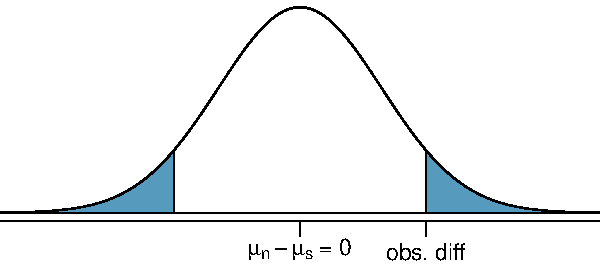
\includegraphics[width=0.6\textwidth]{05/figures/distOfDiffOfSampleMeansForBWOfBabySmokeData/distOfDiffOfSampleMeansForBWOfBabySmokeData}
\end{center}
\end{example}

\begin{example}{Compute the p-value of the hypothesis test using the figure in Example~\exam{pictureOfPValueForEstimateOfDiffOfMeansOfBirthWeights} and evaluate the hypotheses using a significance level of $\alpha=0.05$.} \label{babySmokeHTForWeightComputePValueAndEvalHT}
Since the point estimate is nearly normal, we can find the upper tail using the Z score and normal probability table:
\begin{eqnarray*}
Z = \frac{0.40 - 0}{0.26} = 1.54 \quad \to \quad \text{upper tail } = 1 - 0.938 = 0.062
\end{eqnarray*}
Because this is a two-sided test and we want the area of both tails, we double this single tail to get the p-value: 0.124. This p-value is larger than the significance value, 0.05, so we fail to reject the null hypothesis. There is insufficient evidence to say there is a difference in average birth weight of newborns from mothers who did smoke during pregnancy and newborns from mothers who did not smoke during pregnancy.
\end{example}

\begin{exercise}
Does the conclusion to Example~\exam{babySmokeHTForWeightComputePValueAndEvalHT} mean that smoking and average birth weight are unrelated? Answer in the footnote\footnote{Absolutely not. It is possible that there is some difference but we did not detect it. If this is the case, we made a Type 2 Error.}.
\end{exercise}

\begin{exercise} \label{babySmokeHTIDingHowToDetectDifferences}
If we actually did make a Type 2 Error and there is a difference, what could we have done differently in data collection to be more likely to detect such a difference? Answer in the footnote\footnote{We could have collected larger samples. If the sample size is larger, we tend to have a better shot at finding a difference if one exists.}.
\end{exercise}

\subsection{Summary of inference of the difference of two means}

When considering the difference of two means, there are two common cases: the data observed may be paired or the samples may independent. The first case was treated in Section~\ref{pairedData}, where the one-sample methods were applied to the differences from the paired observations. We examined the second and more complex scenario in this section.

When applying the normal model to the point estimate $\bar{x}_1 - \bar{x}_2$ (corresponding to unpaired data), it is important to verify conditions before applying the inference framework using the normal model. First, each sample mean must meet the conditions for normality; these conditions are described in Chapter~\ref{foundationsForInference} on page~\pageref{terBoxOfCondForXBarBeingNearlyNormalAndSEBeingAccurate}. Secondly, the samples must be collected independently (e.g. not paired data). When these conditions are satisfied, the general inference tools of Chapter~\ref{foundationsForInference} may be applied.

For example, a general confidence interval takes the following form:
\begin{eqnarray*}
\text{point estimate} \pm z^{\star} SE
\end{eqnarray*}
When estimating $\mu_1 - \mu_2$, the point estimate is the difference in sample means, the value $z^{\star}$ corresponds to the confidence level, and the standard error is computed from Equation~(\ref{seOfDifferenceInMeans}) on page~\pageref{seOfDifferenceInMeans}. While the point estimate and standard error formulas change a little, the general framework for a confidence interval stays the same. This is also true in hypothesis tests for differences of means.

In a hypothesis test, we apply the standard framework and use the specific formulas for the point estimate and standard error of a difference in two means. The test statistic represented by the Z score may be computed as
\begin{eqnarray*}
Z = \frac{\text{point estimate} - \text{null value}}{SE}
\end{eqnarray*}
When assessing the difference in two means, the point estimate takes the form $\bar{x}_1 - \bar{x}_2$, and the standard error again takes the form of Equation~(\ref{seOfDifferenceInMeans}) on page~\pageref{seOfDifferenceInMeans}. Finally, the null value is the difference in sample means under the null hypothesis. Just as in Chapter~\ref{foundationsForInference}, the test statistic $Z$ is used to identify the p-value.

\subsection{Examining the standard error formula}

The formula for the standard error of the difference in two means is similar to the formula for other standard errors. Recall that the standard error of a single mean, $\bar{x}_1$, can be approximated by
\begin{eqnarray*}
SE_{\bar{x}_1} = \frac{s_1}{\sqrt{n_1}}
\end{eqnarray*}
where $s_1$ and $n_1$ represent the sample standard deviation and sample size.

The standard error of the difference of two sample means can be constructed from the standard errors of the separate sample means:
\begin{eqnarray}
SE_{\bar{x}_{1} - \bar{x}_{2}}
	= \sqrt{SE_{\bar{x}_1}^2 + SE_{\bar{x}_2}^2}
	= \sqrt{\frac{s_1^2}{{n_1}} + \frac{s_2^2}{{n_2}}}
\label{seOfDiffOfMeansInTermsOfSEOfIndividualMeans}
\end{eqnarray}
This special relationship follows from probability theory.

\begin{exercise} Prerequisite: Section~\ref{randomVariablesSection}.
We can rewrite Equation~(\ref{seOfDiffOfMeansInTermsOfSEOfIndividualMeans}) in a different way:
\begin{eqnarray*}
SE_{\bar{x}_{1} - \bar{x}_{2}}^2 = SE_{\bar{x}_1}^2 + SE_{\bar{x}_2}^2
\end{eqnarray*}
Explain where this formula comes from using the ideas of probability theory. Hint in the footnote\footnote{The standard error squared represents the variance of the estimate. If $X$ and $Y$ are two random variables with variances $\sigma_x^2$ and $\sigma_y^2$, what is the variance of $X-Y$?}.
\end{exercise}


%==========
\section[Comparing many means with ANOVA (special topic)]{Comparing many means with ANOVA\\(special topic)}
\label{anovaAndRegrWithCategoricalVariables}

Fitting and interpreting models using categorical variables as predictors is similar to what we have encountered in simple and multiple regression. However, there is a twist: a single categorical variable will have multiple corresponding parameter estimates. To be precise, if the variable has $C$ categories, then there will be $C-1$ parameter estimates. Furthermore, it is not appropriate to use a Z or T score to determine the significance of the categorical variable as a predictor unless it only has $C=2$ levels.

In this section, we will learn a new method called \term{analysis of variance (ANOVA)} and a new test statistic called $F$. ANOVA is used to assess whether the mean of the outcome variable is different for different levels of a categorical variable:
\begin{itemize}
\setlength{\itemsep}{0mm}
\item[$H_0$:] The mean outcome is the same across all categories. In statistical notation, $\mu_1 = \mu_2 = \cdots = \mu_k$ where $\mu_i$ represents the mean of the outcome for observations in category $i$.
\item[$H_A$:] The mean of the outcome variable is different for some (or all) groups.
\end{itemize}
These hypotheses are used to evaluate a model of the form
\begin{align} 
y_{i,j} = \mu_i + \epsilon_{j} \label{anovaModelForMeans}
\end{align}
where an observation $y_{i,j}$ belongs to group $i$ and has error $\epsilon_j$. Generally we make three assumptions in applying this model:
\begin{itemize}
\setlength{\itemsep}{0mm}
\item the errors are independent,
\item the errors are nearly normal, and
\item the errors have nearly constant variance.
\end{itemize}
These conditions probably look familiar: they are the same conditions we used for multiple regression. When these three assumptions are reasonable, we may perform an ANOVA to determine whether the data provide strong evidence against the null hypothesis that all the $\mu_i$ are equal.

\begin{tipBox}{\tipBoxTitle{Level, category, and group are synonyms}
We sometimes call the levels of a categorical variable its categories or its groups.}
\end{tipBox}

\begin{example}{College departments commonly run multiple lectures of the same introductory course each semester because of high demand. Consider a statistics department that runs three lectures of an introductory statistics course. We might like to determine whether there are statistically significant differences in first exam scores in these three classes ($A$, $B$, and $C$). Describe how the model and hypotheses above could be used to determine whether there are any differences between the three classes.} \label{firstExampleForThreeStatisticsClassesAndANOVA}
The hypotheses may be written in the following form:
\begin{itemize}
\setlength{\itemsep}{0mm}
\item[$H_0$:] The average score is identical in all lectures. Any observed difference is due to chance. Notationally, we write $\mu_A=\mu_B=\mu_C$.
\item[$H_A$:] The average score varies by class. We would reject the null hypothesis in favor of this hypothesis if there were larger differences among the class averages than what we might expect from chance alone.
\end{itemize}
We could label students in the first class as $y_{A,1}$, $y_{A,2}$, $y_{A,3}$, and so on. Students in the second class would be labeled $y_{B,1}$, $y_{B,2}$, etc. And students in the third class: $y_{C,1}$, $y_{C,2}$, etc. Then we could estimate the true averages ($\mu_A$, $\mu_B$, and $\mu_C$) using the group averages: $\bar{y}_{A}$, $\bar{y}_B$, and $\bar{y}_C$.
\end{example}

Strong evidence favoring the alternative hypothesis in ANOVA is described by unusually large differences among the group means. We will soon learn that assessing the variability of the group means relative to the variability among individual observations within each group is key to ANOVA's success.

\begin{example}{Examine Figure~\ref{toyANOVA}. Compare groups I, II, and III. Can you visually determine if the differences in the group centers is due to chance or not? Now compare groups IV, V, and VI. Do these differences appear to be due to chance?}

\begin{figure}[h]
\centering
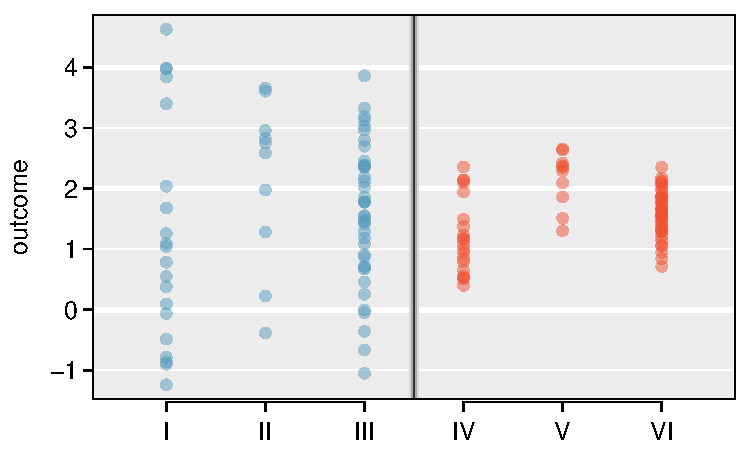
\includegraphics[width=0.75\textwidth]{08/figures/toyANOVA/toyANOVA}
\caption{Side-by-side dot plot for the outcomes for six groups.}
\label{toyANOVA}
\end{figure}

Any real difference in the means of groups I, II, and III is difficult to discern, because the data within each group are very volatile relative to any differences in the average outcome. On the other hand, it appears there are differences in the centers of groups IV, V, and VI. For instance, group IV appears to have a lower mean than that of the other two groups. Investigating groups IV, V, and VI, we see the differences in the groups' centers are noticeable because those differences are large \emph{relative to the variability in the individual observations within each group}.
\end{example}


\subsection{Is batting performance related to player position in MLB?}

We would like to discern whether there are real differences between the batting performance of baseball players according to their position: outfielder (\resp{OF}), infielder (\resp{IF}), designated hitter (\resp{DH}), and catcher (\resp{C}). We will use a data set called \data{mlbBat10}, which includes batting records of 327 Major League Baseball (MLB) players from the 2010 season. Six of the 327 cases represented in \data{mlbBat10} are shown in Table~\ref{mlbBat10DataMatrix}, and descriptions for each variable are provided in Table~\ref{mlbBat10Variables}. The measure we will use for the player batting performance (the outcome variable) is on-base percentage (\var{OBP}). The on-base percentage roughly represents the fraction of the time a player successfully gets on base or hits a home run.

\begin{table}[h]
\centering
\begin{tabular}{rlllrrrrrr}
  \hline
 & name & team & position & AB & H & HR &RBI & AVG & OBP \\ 
  \hline
1 & I Suzuki & SEA & OF & 680 & 214 & 6 & 43 & 0.315 & 0.359 \\ 
  2 & D Jeter & NYY & IF & 663 & 179 & 10 & 67 & 0.270 & 0.340 \\ 
  3 & M Young & TEX & IF & 656 & 186 & 21 & 91 & 0.284 & 0.330 \\ 
  $\vdots$ & $\vdots$ & $\vdots$ & $\vdots$ & $\vdots$ & $\vdots$ & $\vdots$ & $\vdots$ \\
  325 & B Molina & SF & C & 202 & 52 & 3 & 17 & 0.257 & 0.312 \\ 
  326 & J Thole & NYM & C & 202 & 56 & 3 & 17 & 0.277 & 0.357 \\ 
  327 & C Heisey & CIN & OF & 201 & 51 & 8 & 21 & 0.254 & 0.324 \\ 
   \hline
\end{tabular}
\caption{Six cases from the \data{mlbBat10} data matrix.}
\label{mlbBat10DataMatrix}
\end{table}

\begin{table}
\centering\small
\begin{tabular}{lp{9.5cm}}
\hline
{\bf variable} & {\bf description} \\
\hline
%\begin{itemize}
\var{name} & Player name \\
\var{team} & The player's team, where the team names are abbreviated \\
\var{position} & The player's primary field position (\resp{OF}, \resp{IF}, \resp{DH}, \resp{C}) \\
\var{AB} & Number of opportunities at bat \\
\var{H} & Number of hits \\
\var{HR} & Number of home runs \\
\var{RBI} & Number of runs batted in \\
\var{batAverage} & Batting average, which is equal to $\resp{H}/\resp{AB}$ \\
\hline
\end{tabular}
\caption{Variables and their descriptions for the \data{mlbBat10} data set.}
\label{mlbBat10Variables}
\end{table}

\begin{exercise} \label{nullHypForOBPAgainstPosition}
The null hypothesis under consideration is the following: $\mu_{\resp{OF}} = \mu_{\resp{IF}} = \mu_{\resp{DH}} = \mu_{\resp{C}}$.
Write the null and corresponding alternative hypotheses in plain language. Answers in the footnote\footnote{$H_0$: The average on-base percentage is equal across the four positions. $H_A$: The average on-base percentage varies across some (or all) groups.}.
\end{exercise}

\begin{example}{The player positions have been divided into four groups: outfield (\resp{OF}), infield (\resp{IF}), designated hitter (\resp{DH}), and catcher (\resp{C}). What would be an appropriate point estimate of the batting average by outfielders, $\mu_{\resp{OF}}$?}
A good estimate of the batting average by outfielders would be the sample average of \var{batAverage} for just those players whose position is outfield: $\bar{y}_{OF} = 0.334$.
\end{example}

Table~\ref{mlbHRPerABSummaryTable} provides summary statistics for each group. A side-by-side box plot for the batting average is shown in Figure~\ref{mlbANOVABoxPlot}. Notice that the variability appears to be approximately constant across groups; nearly constant variance across groups is an important assumption that must be satisfied before we consider the ANOVA approach.

\begin{table}[ht]
\centering\small
\begin{tabular}{lrrrr}
\hline
	& \resp{OF} & \resp{IF} & \resp{DH} & \resp{C} \\
\hline
Sample size ($n_i$)	& 120 & 154 & 14 & 39 \\
Sample mean ($\bar{y}_i$)	& 0.334 & 0.332 & 0.348 & 0.323 \\
Sample SD ($s_i$)	& 0.029 & 0.037 & 0.036 & 0.045 \\
\hline
\end{tabular}
\caption{Summary statistics of on-base percentage, split by player position.}
\label{mlbHRPerABSummaryTable}
\end{table}

\begin{figure}
\centering
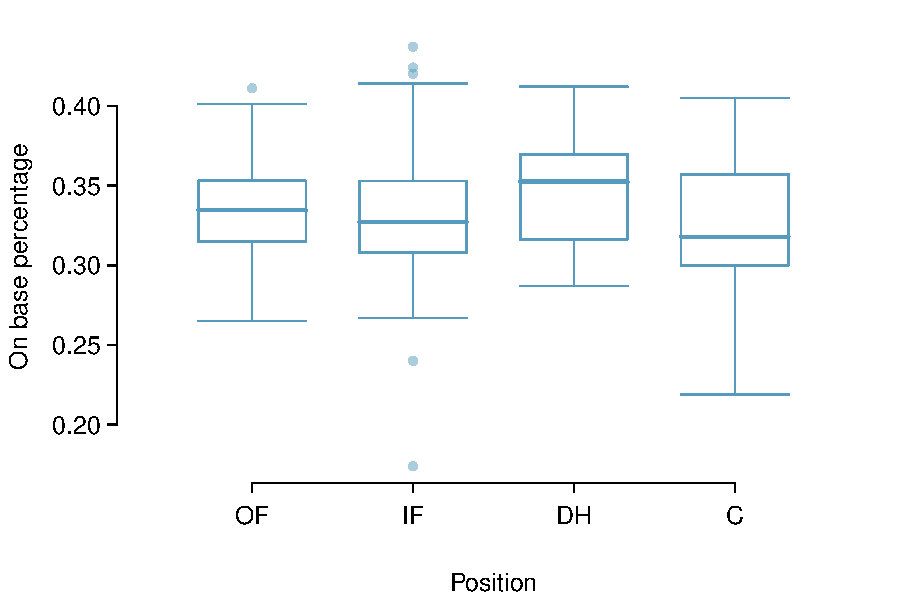
\includegraphics[width=0.85\textwidth]{08/figures/mlbANOVA/mlbANOVABoxPlot}
\caption{Side-by-side box plot of the on-base percentage for 327 players across four groups.}
\label{mlbANOVABoxPlot}
\end{figure}

\begin{example}{The largest difference between the sample means is between the designated hitter and the catcher positions. Consider again the original hypotheses:
\begin{itemize}
\setlength{\itemsep}{0mm}
\item[$H_0$:] $\mu_{\resp{OF}} = \mu_{\resp{IF}} = \mu_{\resp{DH}} = \mu_{\resp{C}}$
\item[$H_A$:] The average on-base percentage ($\mu_i$) varies across some (or all) groups.
\end{itemize}
Why might it be inappropriate to run the test by simply estimating whether the difference of $\mu_{\var{DH}}$ and $\mu_{\resp{C}}$ is statistically significant at a 0.05 significance level?}
\label{multipleComparisonExampleThatIncludesDiscussionOfClassrooms}
The primary issue here is that we are inspecting the data before picking the groups that will be compared. It is inappropriate to examine all data by eye (informal testing) and only afterwards decide which parts to formally test. This is called \term{data snooping} or \term{data fishing}. Naturally we would pick the groups with the large differences for the formal test, leading to an unintentional inflation in the Type 1 Error rate. To understand this better, let's consider a slightly different problem.

Suppose we are to measure the aptitude for students in 20 classes in a large elementary school at the beginning of the year. In this school, all students are randomly assigned to classrooms, so any differences we observe between the classes at the start of the year are completely due to chance. However, with so many groups, we will probably observe a few groups that look rather different from each other. If we select only these classes that look so different, we will probably make the wrong conclusion that the assignment wasn't random. While we might only formally test differences for a few pairs of classes, we informally evaluated the other classes by eye before choosing the most extreme cases for a comparison.
\end{example}

For additional reading on the ideas expressed in Example~\ref{multipleComparisonExampleThatIncludesDiscussionOfClassrooms}, we recommend reading about the \term{prosecutor's fallacy}\footnote{See, for example, \url{http://www.stat.columbia.edu/~cook/movabletype/archives/2007/05/the_prosecutors.html}.}.

In the next section we will learn how to use the $F$ statistic and ANOVA to test whether differences in means could have happened just by chance.


\subsection{Analysis of variance (ANOVA) and the F test}

The method of analysis of variance focuses on answering one question: is the variability in the sample means so large that it seems unlikely to be from chance alone? This question is different from earlier testing procedures since we will \emph{simultaneously} consider many groups, and evaluate whether their sample means differ more than we would expect from natural variation. We call this variability the \term{mean square between groups ($MSG$)}, and it has an associated degrees of freedom, $df_{G}=k-1$ when there are $k$ groups. The $MSG$ is sort of a scaled variance formula for means. If the null hypothesis is true, any variation in the sample means is due to chance and shouldn't be too large%; it should be roughly equal to the variability in the outcome variable
. Details of $MSG$ calculations are provided in the footnote\footnote{Let $\bar{y}$ represent the mean of outcomes across all groups. Then the mean square between groups is computed as
\begin{align*}
MSG = \frac{1}{df_{G}}SSG = \frac{1}{k-1}\sum_{i=1}^{k} n_{i}\left(\bar{y}_{i} - \bar{y}\right)^2
\end{align*}
where $SSG$ is called the \term{sum of squares between groups} and $n_{i}$ is the sample size of group $i$.}, however, we typically use software for these computations.

The mean square between the groups is, on its own, quite useless in a hypothesis test. We need a benchmark value for how much variability should be expected among the sample means if the null hypothesis is true. To this end, we compute the mean of the squared errors, often abbreviated as the \term{mean square error ($MSE$)}, which has an associated degrees of freedom value $df_E=n-k$. It is helpful to think of $MSE$ as a measure of the variability of the residuals. Details of the computations of the $MSE$ are provided in the footnote\footnote{Let $\bar{y}$ represent the mean of outcomes across all groups. Then the \term{sum of squares total ($SST$)} is computed as
\begin{align*}
SST = \sum_{i=1}^{n} \left(y_{i} - \bar{y}\right)^2
\end{align*}
where the sum is over all observations in the data set. Then we compute the \term{sum of squared errors ($SSE$)} in one of three equivalent ways:
\begin{align*}
SSE &= SST - SSG \\
	&= (n_1-1)s_1^2 + (n_2-1)s_2^2 + \cdots + (n_k-1)s_k^2 \\
	&= \sum_{j=1}^{n} e_i^2
\end{align*}
where $s_i^2$ is the sample variance (square of the standard deviation) of the residuals in group $i$, and the last expression represents the sum of the squared residuals across all groups. Then the $MSE$ is the standardized form of $SSE$: $MSE = \frac{1}{df_{E}}SSE$.} for the interested reader.

When the null hypothesis is true, any differences among the sample means are only due to chance, and the $MSG$ and $MSE$ should be about equal. As a test statistic for ANOVA, we examine the fraction of $MSG$ and $MSE$:
\begin{align} \label{formulaForTheFStatistic}
F = \frac{MSG}{MSE}
\end{align}
The $MSG$ represents a measure of the between-group variability, and $MSE$ the variability within each of the groups.

\begin{exercise}
For the baseball data, $MSG = 0.00252$ and $MSE=0.00127$. Identify the degrees of freedom associated with each mean square and verify the $F$ statistic is 1.994.
\end{exercise}

We use the $F$ statistic to evaluate the hypotheses in what is called an \term{F test}. We compute a p-value from the $F$ statistic using an $F$ distribution, which has two associated parameters: $df_{1}$ and $df_{2}$. For the $F$ statistic in ANOVA, $df_{1} = df_{G}$ and $df_{2}= df_{E}$. An $F$ distribution with 3 and 323 degrees of freedom, corresponding to the $F$ statistic for the baseball hypothesis test, is shown in Figure~\ref{fDist3And323}.

\begin{figure}[ht]
\centering
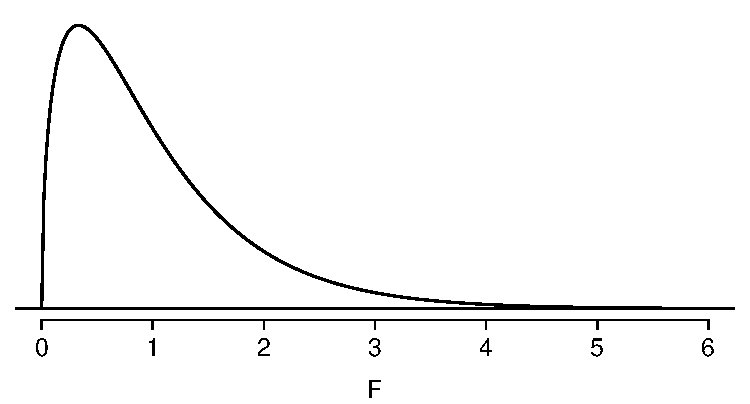
\includegraphics[width=0.7\textwidth]{08/figures/fDist3And323/fDist3And323}
\caption{An $F$ distribution with $df_1=3$ and $df_2=323$.}
\label{fDist3And323}
\end{figure}

The larger the observed variability in the sample means ($MSG$) relative to the residuals ($MSE$), the larger $F$ will be and the stronger the evidence against the null hypothesis. Because larger values of $F$ represent stronger evidence against the null hypothesis, we use the upper tail of the distribution to compute a p-value.

\begin{termBox}{\tBoxTitle{The $F$ statistic and the $F$ test}
Analysis of variance (ANOVA) is used to test whether the mean outcome differs across 2 or more groups. ANOVA uses a test statistic $F$, which represents a standardized ratio of variability in the sample means relative to the variability of the residuals. If $H_0$ is true and the model assumptions are satisfied, the statistic $F$ follows an $F$ distribution with parameters $df_{1}=k-1$ and $df_{2}=n-k$. The upper tail of the $F$ distribution is used to represent the p-value.}
\end{termBox}

\begin{exercise}\label{describePValueAreaForFDistributionInMLBOBPExample}
The test statistic for the baseball example is $F=1.994$. Shade the area corresponding to the p-value in Figure~\ref{fDist3And323}.
\end{exercise}

\begin{example}{The p-value corresponding to the solution for Exercise~\ref{describePValueAreaForFDistributionInMLBOBPExample} is equal to about 0.115. Does this provide strong evidence against the null hypothesis?}
The p-value is larger than 0.05, indicating the evidence is not sufficiently strong to reject the null hypothesis at a significance level of 0.05. That is, the data do not provide strong evidence that the average on-base percentage varies by player's primary field position.
\end{example}


\subsection{Reading an ANOVA table from software}

The calculations required to perform an ANOVA by hand are tedious and prone to human error. For these reasons it is common to use a statistical software to calculate the $F$ statistic and p-value.

An ANOVA can be summarized in a table very similar to that of a regression summary. Table~\ref{anovaSummaryTableForOBPAgainstPosition} shows an ANOVA summary to test whether the mean of on-base percentage varies by player positions in the MLB.

\begin{table}[ht]
\centering
\begin{tabular}{lrrrrr}
  \hline
 & Df & Sum Sq & Mean Sq & F value & Pr($>$F) \\ 
  \hline
position & 3 & 0.0076 & 0.0025 & 1.9943 & 0.1147 \\ 
  Residuals & 323 & 0.4080 & 0.0013 &  &  \\    \hline
\multicolumn{6}{r}{$s_{pooled} = 0.036$ on $df=323$}
\end{tabular}
\caption{ANOVA summary for testing whether the average on-base percentage differs across player positions.}
\label{anovaSummaryTableForOBPAgainstPosition}
\end{table}

\begin{exercise}
Earlier you verified that the $F$ statistic for this analysis was 1.994, and the p-value of 0.115 was provided. Circle these values in Table~\ref{anovaSummaryTableForOBPAgainstPosition} and notice the corresponding column name. Notice that both of these values are in the row labeled \emph{position}, which corresponds to the categorical variable representing the player position variable.
\end{exercise}

\begin{exercise}
The $s_{pooled}=0.036$ on $df=323$ describes the estimated standard deviation associated with the residuals. Verify that $s_{pooled}$ equals the square root of the $MSE$ for the \emph{Residuals} row.
\end{exercise}


\subsection{Graphical diagnostics for an ANOVA analysis}

There are three primary conditions we must check for an ANOVA analysis, all related to the residuals (errors) associated with the model. Recall that we assume the errors are independent, nearly normal, and have nearly constant variance across the groups.

\begin{description}
\item[Independence.] If observations are collected in a particular order, we should plot the residuals in the order the corresponding observations were collected (e.g. see Figure~\ref{mkDiagnosticInOrder} on page~\pageref{mkDiagnosticInOrder}). For the baseball data, the data were collected from a sorted table, making such a review impossible. However, we can consider the nature of the data: Do we have reason to believe players are not independent? There are not obvious reasons why independence should not hold, so we will assume independence is reasonable in lieu of being able to examine this condition using data.
\item[Approximately normal.] The normality assumption for the residuals is especially important when the sample size is quite small. Figure~\ref{mlbANOVADiagNormality} shows a normal probability plot for the residuals from the baseball data. We do see some deviation from normality at the low end, where there is a longer tail than what we would expect if the residuals were truly normal. While we should report this finding with the results of the hypothesis test, this slight deviation probably has little impact on the test results since there are so many players included in the sample and they are not spread thinly across many groups. % but can be slightly relaxed for residuals of groups with larger sample sizes. We do see some deviations from normality in the lower tail. However, the three smallest residuals are from the infield and outfield groups. Because each of these groups each contain over 100 cases, so the potential outliers probably alright (but these observations are worth mentioning in a report of the analysis).

\begin{figure}
\centering
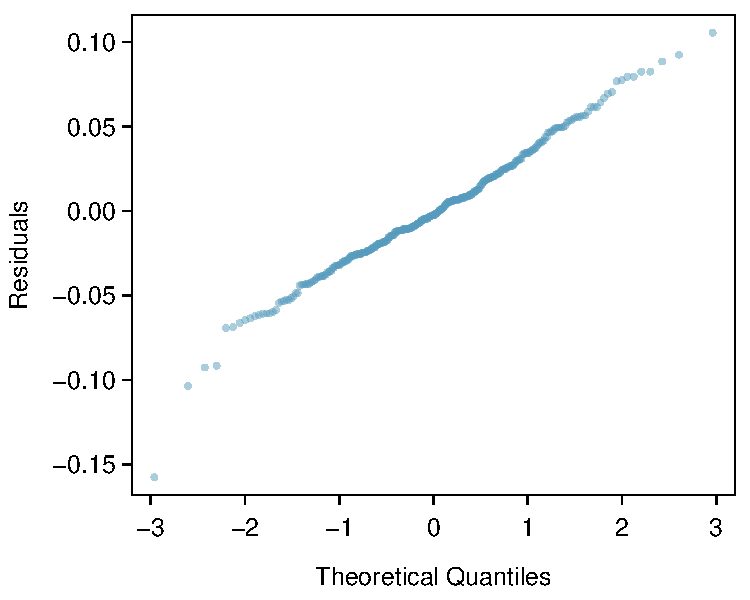
\includegraphics[width=0.75\textwidth]{08/figures/mlbANOVA/mlbANOVADiagNormality}
\caption{Normal probability plot of the residuals.}
\label{mlbANOVADiagNormality}
\end{figure}

\item[Constant variance.] The last assumption is that the variance associated with the residuals is nearly constant from one group to the next. This assumption can be checked by examining a side-by-side box plot of the outcomes, as in Figure~\ref{mlbANOVABoxPlot}. In this case, the variability is similar in the four groups but not identical. We see in Table~\ref{mlbHRPerABSummaryTable} on page~\pageref{mlbHRPerABSummaryTable} that the standard deviation varies a bit from one group to the next. Whether these differences are from natural variation is unclear, so we should report this uncertainty with the final results.
\end{description}

\begin{caution}
{Diagnostics for an ANOVA analysis}
{Independence is always important to an ANOVA analysis. The normality condition is very important when the sample sizes for each group are relatively small. The constant variance condition is especially important when the sample sizes differ between groups.}
\end{caution}


\subsection{Multiple comparisons and controlling Type 1 Error rate}

\label{multipleComparisonsAndControllingTheType1ErrorRate}

When we reject the null hypothesis in an ANOVA analysis, we might wonder, which of these groups have different means? To answer this question, we compare the means of each possible pair of groups. For instance, if there are three groups and there is strong evidence that there are some differences in the group means, there are three comparisons to make: group 1 to group 2, group 1 to group 3, and group 2 to group 3. These comparisons can be accomplished using a two-sample $t$ test, but we must use a modified significance level and a pooled estimate of the standard deviation across groups.

\begin{example}{Example~\ref{firstExampleForThreeStatisticsClassesAndANOVA} on page~\pageref{firstExampleForThreeStatisticsClassesAndANOVA} discussed three statistics lectures, all taught during the same semester. Table~\ref{summaryStatisticsForClassTestData} shows summary statistics for these three courses, and a side-by-side box plot of the data is shown in Figure~\ref{classDataSBSBoxPlot}. We would like to conduct an ANOVA for these data. Do you see any deviations from the three conditions for ANOVA?}
In this case (like many others) it is difficult to check independence in a rigorous way. Instead, the best we can do is use common sense to consider reasons the assumption of independence may not hold. For instance, the independence assumption may not be reasonable if there is a star teaching assistant that only half of the students may access; such a scenario would divide a class into two subgroups. After carefully considering the data, we believe that assuming independence may be acceptable.

The distributions in the side-by-side box plot appear to be roughly symmetric and show no noticeable outliers.

The box plots show approximately equal variability, which can be verified in Table~\ref{summaryStatisticsForClassTestData}, supporting the constant variance assumption.
\end{example}

\begin{table}[ht]
\centering
\begin{tabular}{lrrr}
  \hline
Class $i$	& A	& B	& C \\ 
  \hline
$n_i$		& 58	& 55	& 51 \\ 
$\bar{y}_i$	& 75.1	& 72.0	& 78.9 \\ 
$s_i$		& 13.9	& 13.8	& 13.1 \\ 
\hline
\end{tabular}
\caption{Summary statistics for the first midterm scores in three different lectures of the same course.}
\label{summaryStatisticsForClassTestData}
\end{table}

\begin{figure}[ht]
\centering
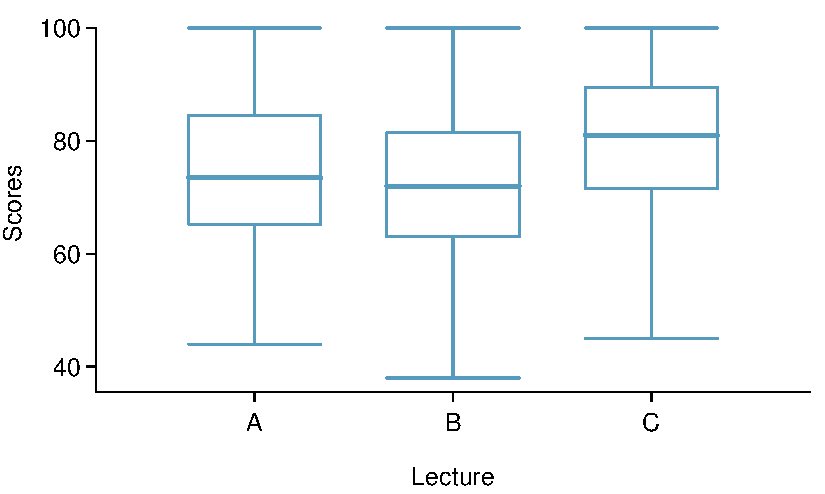
\includegraphics[width=0.8\textwidth]{08/figures/classData/classDataSBSBoxPlot}
\caption{Side-by-side box plot for the first midterm scores in three different  lectures of the same course.}
\label{classDataSBSBoxPlot}
\end{figure}

\begin{exercise} \label{exerExaminingAnovaSummaryTableForMidtermData}
An ANOVA was conducted for the midterm data, and a summary is shown in Table~\ref{anovaSummaryTableForMidtermData}. What should we conclude?
\end{exercise}

\begin{table}[ht]
\centering
\begin{tabular}{lrrrrr}
  \hline
 & Df & Sum Sq & Mean Sq & F value & Pr($>$F) \\ 
  \hline
lecture & 2 & 1290.11 & 645.06 & 3.48 & 0.0330 \\ 
  Residuals & 161 & 29810.13 & 185.16 &  &  \\ 
   \hline
\multicolumn{6}{r}{$s_{pooled}=13.61$ on $df=161$}
\end{tabular}
\caption{ANOVA summary table for the midterm data.}
\label{anovaSummaryTableForMidtermData}
\end{table}

There is strong evidence that the different means in each of the three classes is not simply due to chance. We might wonder, which of the classes are actually different? As discussed in earlier chapters, a two-sample $t$ test could be used to test for differences in each possible pair of groups. However, one pitfall was discussed in Example~\ref{multipleComparisonExampleThatIncludesDiscussionOfClassrooms} on page~\pageref{multipleComparisonExampleThatIncludesDiscussionOfClassrooms}: when we run so many tests, the Type~1 Error rate increases. This issue is resolved by using a modified significance level.

\begin{termBox}{\tBoxTitle{Multiple comparisons and the Bonferroni correction for $\alpha$}
The scenario of testing many pairs of groups is called \term{multiple comparisons}. The \term{Bonferroni correction} suggests that a more stringent significance level is more appropriate for these tests:
\begin{align*}
\alpha^* = \alpha / K
\end{align*}
where $K$ is the number of comparisons being considered (formally or informally). If there are $k$ groups, then usually all possible pairs are compared and $K=\frac{k(k-1)}{2}$.}
\end{termBox}

\begin{example}{In Exercise~\ref{exerExaminingAnovaSummaryTableForMidtermData}, you found that the data showed strong evidence of differences in the average midterm grades between the three lectures. Complete the three possible pairwise comparisons using the Bonferroni correction and report any differences.} \label{multipleComparisonsOfThreeStatClasses}
We use a modified significance level of $\alpha^* = 0.05/3 = 0.0167$. Additionally, we use the pooled estimate of the standard deviation: $s_{pooled}=13.61$ on $df=161$.

Lecture A versus Lecture B: The estimated difference and standard error are, respectively,
\begin{align*}
\bar{y}_A - \bar{y}_{B} &= 75.1 - 72 = 3.1
	&SE = \sqrt{\frac{13.61^2}{58} + \frac{13.61^2}{55}} &= 2.56
\end{align*}
(See Section~\ref{pooledStandardDeviations} on page~\ref{pooledStandardDeviations} for additional details.) This results in a $T$ score of 1.21 on $df = 161$ (we use the $df$ associated with $s_{pooled}$) and a two-tailed p-value of 0.228. This p-value is larger than $\alpha^*=0.0167$, so there is not strong evidence of a difference in the means of lectures A and B.

Lecture A versus Lecture C: The estimated difference and standard error are 3.8 and 2.61, respectively. This results in a $T$ score of 1.46 on $df = 161$ and a two-tailed p-value of 0.1462. This p-value is larger than $\alpha^*$, so there is not strong evidence of a difference in the means of lectures A and C.

Lecture B versus Lecture C: The estimated difference and standard error are 6.9 and 2.65, respectively. This results in a $T$ score of 2.60 on $df = 161$ and a two-tailed p-value of 0.0102. This p-value is smaller than $\alpha^*$. Here we find strong evidence of a difference in the means of lectures B and C.
\end{example}

We might summarize the findings of the analysis from Example~\ref{multipleComparisonsOfThreeStatClasses} using the following notation:
\begin{align*}
\mu_A &\stackrel{?}{=} \mu_B
	&\mu_A &\stackrel{?}{=} \mu_C
	&\mu_B &\neq \mu_C
\end{align*}
The midterm mean in lecture A is not statistically distinguishable from those of lectures B or C. However, there is strong evidence that lectures B and C are different. In the first two pairwise comparisons, we did not have sufficient evidence to reject the null hypothesis. Recall that failing to reject $H_0$ does not imply $H_0$ is true.

\begin{caution}
{Sometimes an ANOVA will reject the null but no groups will have statistically significant differences}
{It is possible to reject the null hypothesis using ANOVA and then to not subsequently identify differences in the pairwise comparisons. However, \emph{this does not invalidate the ANOVA conclusion}. It only means we have not been able to successfully identify which groups differ in their means.}
\end{caution}

The ANOVA procedure examines the big picture: it considers all groups simultaneously to decipher whether there is evidence that some difference exists. Even if the test indicates that there is strong evidence of differences in group means, identifying with high confidence a specific difference as statistically significant is more difficult.

Consider the following analogy: we observe a Wall Street firm that makes large quantities of money based on predicting mergers. Mergers are generally difficult to predict, and if the prediction success rate is extremely high, that may be considered sufficiently strong evidence to warrant investigation by the Securities and Exchange Commission (SEC). While the SEC may be quite certain that there is insider trading taking place at the firm, the evidence against any single trader may not be very strong. It is only when the SEC considers all the data that they identify the pattern. This is effectively the strategy of ANOVA: stand back and consider all the groups simultaneously.


